\documentclass[10pt]{beamer}
\usetheme[
%%% options passed to the outer theme
%    hidetitle,           % hide the (short) title in the sidebar
%    hideauthor,          % hide the (short) author in the sidebar
%    hideinstitute,       % hide the (short) institute in the bottom of the sidebar
%    shownavsym,          % show the navigation symbols
%    width=2cm,           % width of the sidebar (default is 2 cm)
%    hideothersubsections,% hide all subsections but the subsections in the current section
%    hideallsubsections,  % hide all subsections
    left               % right of left position of sidebar (default is right)
%%% options passed to the color theme
%    lightheaderbg,       % use a light header background
  ]{AAUsidebar}

% If you want to change the colors of the various elements in the theme, edit and uncomment the following lines
% Change the bar and sidebar colors:
%\setbeamercolor{AAUsidebar}{fg=red!20,bg=red}
%\setbeamercolor{sidebar}{bg=red!20}
% Change the color of the structural elements:
%\setbeamercolor{structure}{fg=red}
% Change the frame title text color:
%\setbeamercolor{frametitle}{fg=blue}
% Change the normal text color background:
%\setbeamercolor{normal text}{bg=gray!10}
% ... and you can of course change a lot more - see the beamer user manual.

%\usepackage{graphicx}
%\usepackage{caption}
%\usepackage{subcaption}

\usepackage[utf8]{inputenc}
\usepackage[english]{babel}
\usepackage[T1]{fontenc}
% Or whatever. Note that the encoding and the font should match. If T1
% does not look nice, try deleting the line with the fontenc.
\usepackage{helvet}
\usepackage{subfigure}

% colored hyperlinks
\newcommand{\chref}[2]{%
  \href{#1}{{\usebeamercolor[bg]{AAUsidebar}#2}}%
}

\title[Double Tracking Antennas for UAS Communication]% optional, use only with long paper titles
{Double Tracking Antennas for UAS Communication}

\subtitle{Control and Automation}  % could also be a conference name

\date{\today}

\author[Group CA832] % optional, use only with lots of authors
{
  Group CA832\\
  \href{mailto:16gr832@es.aau.dk}{{\tt {16gr832}@student.aau.dk}}
}
% - Give the names in the same order as they appear in the paper.
% - Use the \inst{?} command only if the authors have different
%   affiliation. See the beamer manual for an example

\institute[
%  {\includegraphics[scale=0.2]{aau_segl}}\\ %insert a company, department or university logo
  Dept.\ of Electronics and IT\\
  Aalborg University\\
  Denmark
] % optional - is placed in the bottom of the sidebar on every slide
{% is placed on the title page
  Department of Electronics and IT\\
  Aalborg University\\
  Denmark
  
  %there must be an empty line above this line - otherwise some unwanted space is added between the university and the country (I do not know why;( )
}


% specify a logo on the titlepage (you can specify additional logos an include them in 
% institute command below
\pgfdeclareimage[height=1.5cm]{titlepagelogo}{AAUgraphics/aau_logo_new} % placed on the title page
%\pgfdeclareimage[height=1.5cm]{titlepagelogo2}{graphics/aau_logo_new} % placed on the title page
\titlegraphic{% is placed on the bottom of the title page
  \pgfuseimage{titlepagelogo}
%  \hspace{1cm}\pgfuseimage{titlepagelogo2}
}


\begin{document}
% the titlepage
{\aauwavesbg%
\begin{frame}[plain,noframenumbering] % the plain option removes the sidebar and header from the title page
  \titlepage
\end{frame}}
%%%%%%%%%%%%%%%%


\section{Introduction}

\begin{frame}{Introduction}{}
\begin{figure}[H]
\centerline{
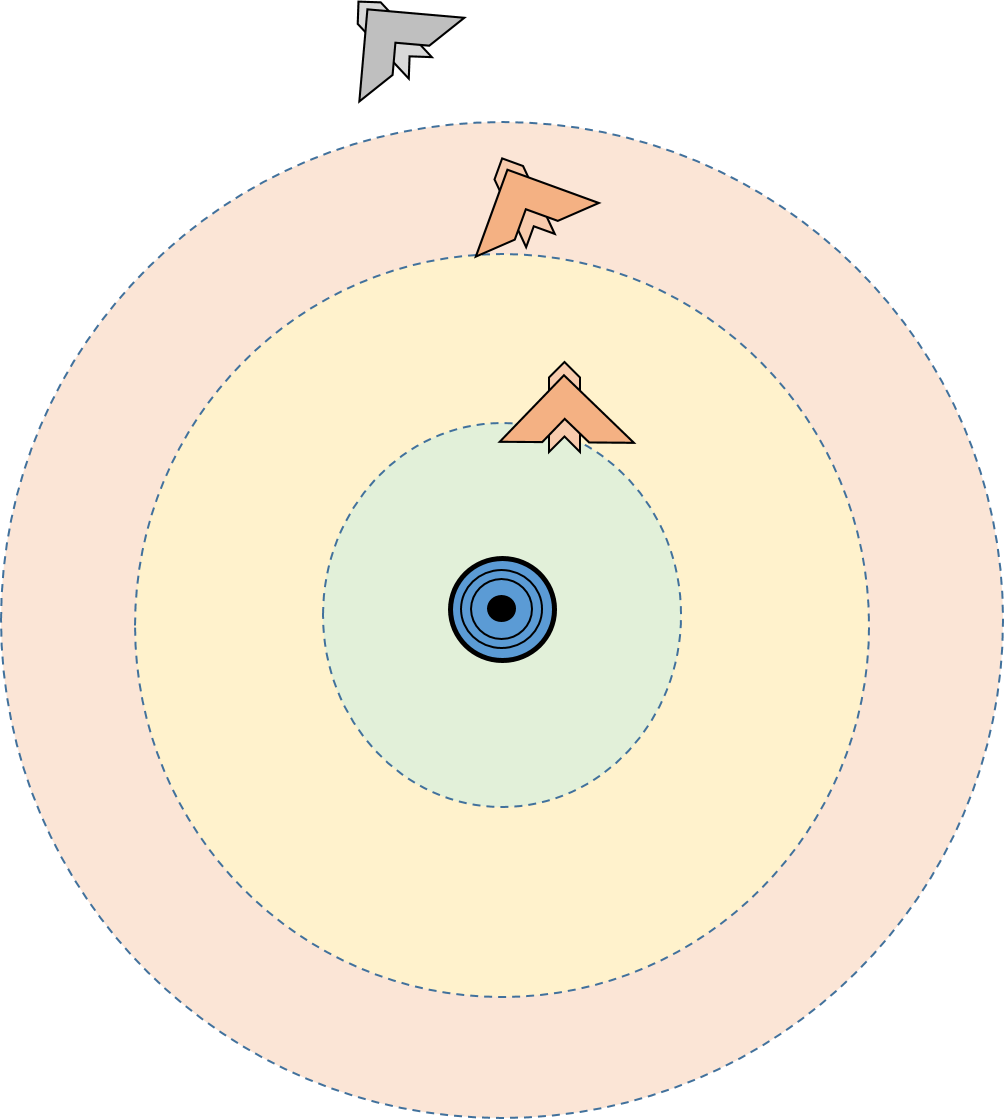
\includegraphics[scale=0.35]{figures/intro.png}}
\label{fig:overview}
\end{figure}
\end{frame}



% TOC
\begin{frame}{Agenda}{}
\tableofcontents
\end{frame}
%%%%%%%%%%%%%%%%

\section{Overview}
\subsection{Hardware}

\begin{frame}{Hardware}{}
  \begin{block}{Unmanned Aicraft System (UAS)}
    \begin{enumerate}
      \item Unmanned Aircraft (UA)
      \item Ground Station (GS)
      \item Antennas
      \item DC Servomotor
    \end{enumerate}
  \end{block}
\end{frame}


\chapter{Frames}\label{ch:frames}

In navigation, guidance, and control of an aircraft or rotorcraft, there are several
coordinate systems (or frames) intensively used in design and analysis. For ease of references, in this chapter the coordinate systems adopted in this project have been sumarized, which include:

\begin{itemize}
\item{The Geodetic Coordinate System}
\item{The Earth-Centered Earth-Fixed (ECEF) Coordinate System}
\item{The local North-East-Down (NED) Coordinate System}
\item{The vehicle-carried NED Coordinate System}
\item{The Body Coordinate System}
\end{itemize}

The relationships among these coordinate systems, i.e., the coordinate transformations, are also introduced. We need to point out that small UAs are normally used at low speeds in relatively small regions (non trans-oceanic travels), due to their inherent mechanical design and power limitation. This is crucial to some simplifications made in the coordinate transformation, e.g., omitting unimportant items in the transformation between the local NED frame and the body frame. For the same reason, partial transformation relationships provided in this chapter are not suitable for describing flight situations in which the rotation of the Earth is taken into account.
\subsection{Telecommunication}

\begin{frame}{Telecommunication}{}

  \begin{block}{Line-Of-Sight (LOS) Propagation}

  \end{block}
  
  \begin{block}{Link Budget}

  \end{block}

  \begin{block}{Fresnel Zones}

  \end{block}

  \begin{block}{MAVLink Protocol}

  \end{block}

\end{frame}


\section{Methods}
\chapter{Modelling}\label{ch:model}

!!! INTRO !!!

??? State-space model ???


%
%\begin{frame}{Controller}{}
%
%  \begin{block}{PID}
%
%  \end{block}
%  
%  \begin{block}{Tunning}
%
%  \end{block}
%
%  \begin{block}{Comparion}
%
%  \end{block}
%
%\end{frame}

%Overview
\begin{frame}{Modelling}{Moving Angle System}
  \begin{block}{Moving Angle System:}

	  \begin{itemize}
  	  	\item Servomotor
	  	\item Gear
	  	\item Sensor
	  	\item Controller
	  	\item Saturation
	  \end{itemize}

	  \begin{figure}
        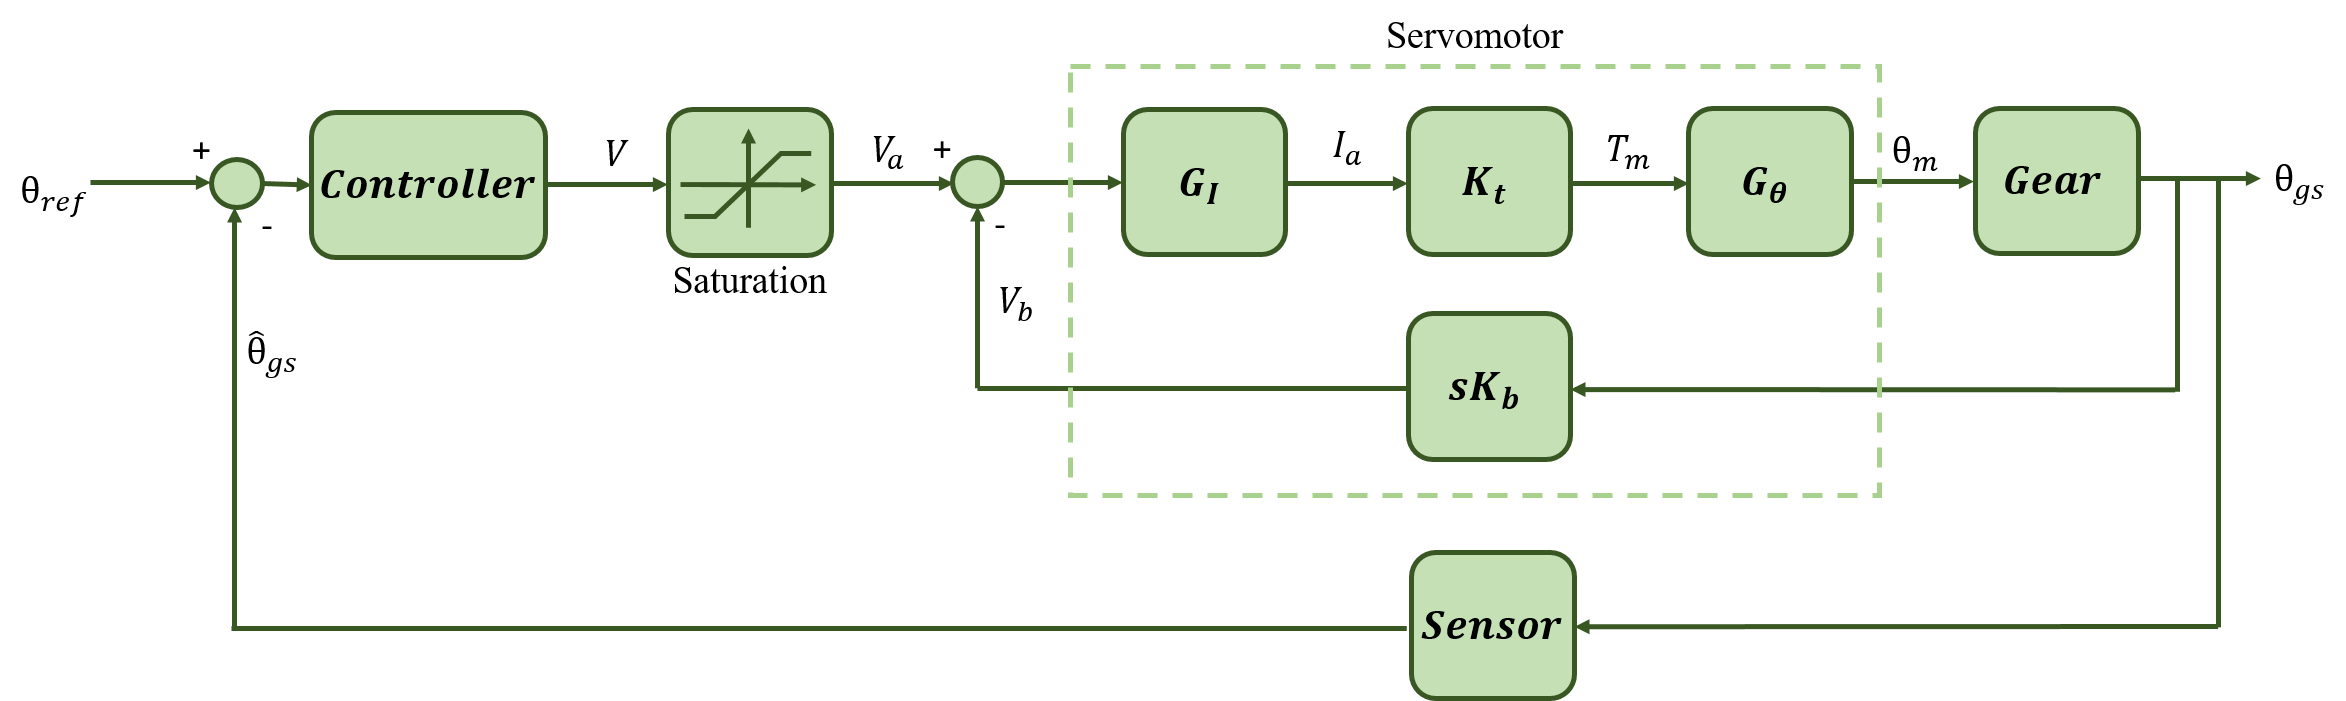
\includegraphics[scale=0.24]{../report/figures/complete_model.png}
      \end{figure}
  
  \end{block}
\end{frame}


%Servomotor
\begin{frame}{Modelling}{Moving Angle System}
  \begin{block}{Moving Angle System:}

	  \begin{itemize}
	  	\item Servomotor - modelled
	  \end{itemize}

	  \begin{figure}
        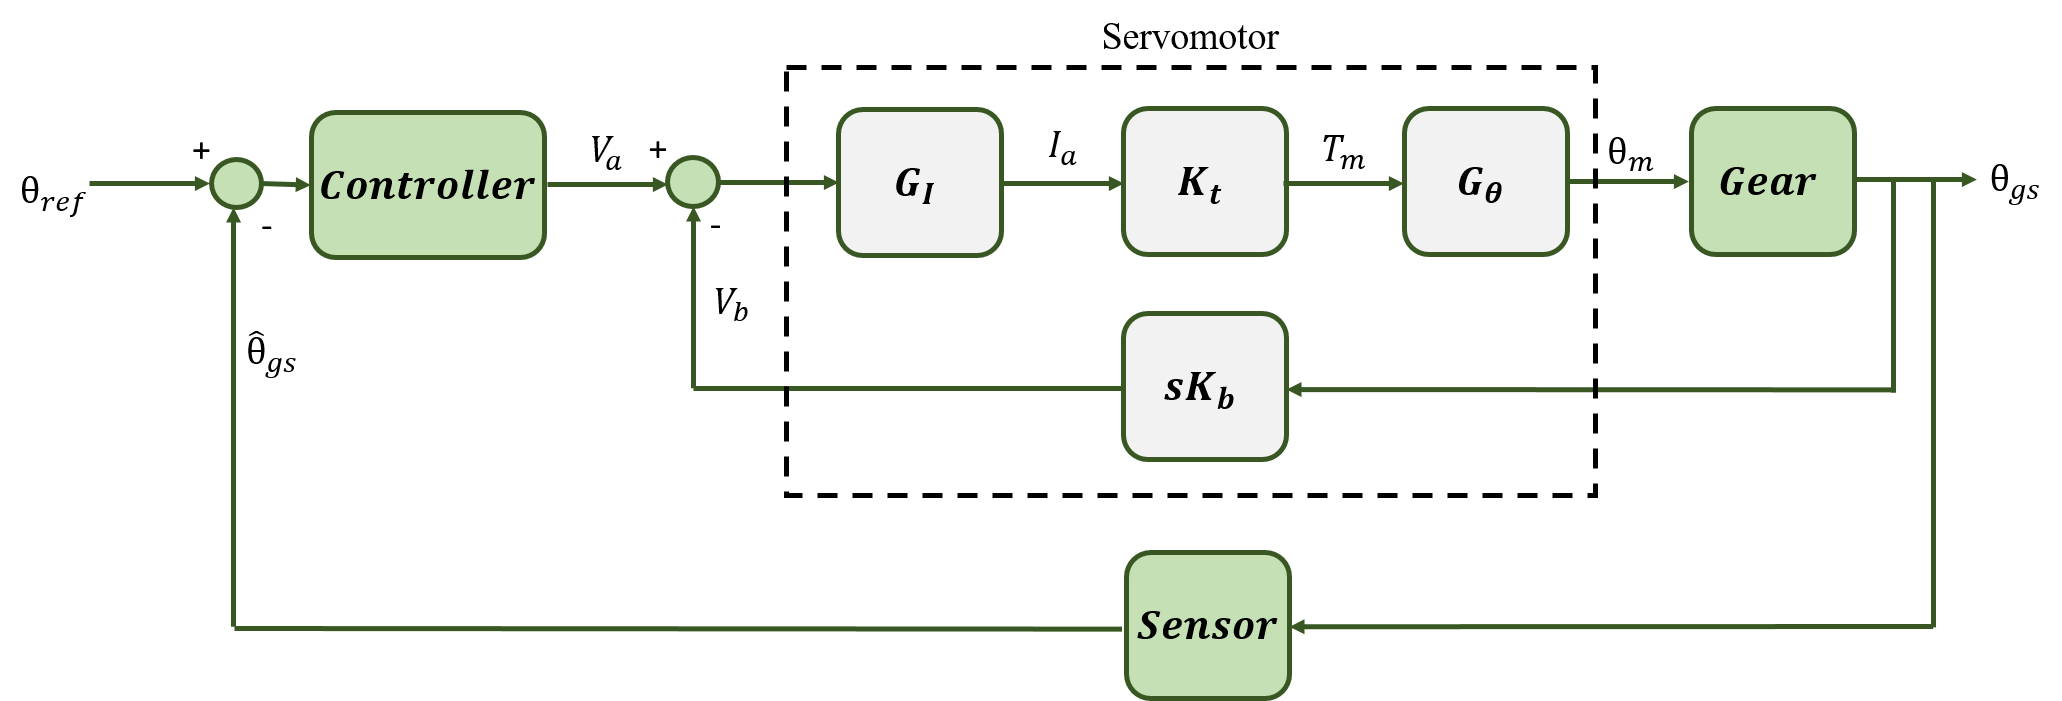
\includegraphics[scale=0.24]{../report/figures/servo+gear+noise+servomotor.png}
      \end{figure}
  
  \end{block}
\end{frame}

%Gear
\begin{frame}{Modelling}{Moving Angle System}
  \begin{block}{Moving Angle System:}
	  \begin{itemize}
	  	\item Gear - reduce speed and increase precision
	  \end{itemize}
	  \begin{figure}
        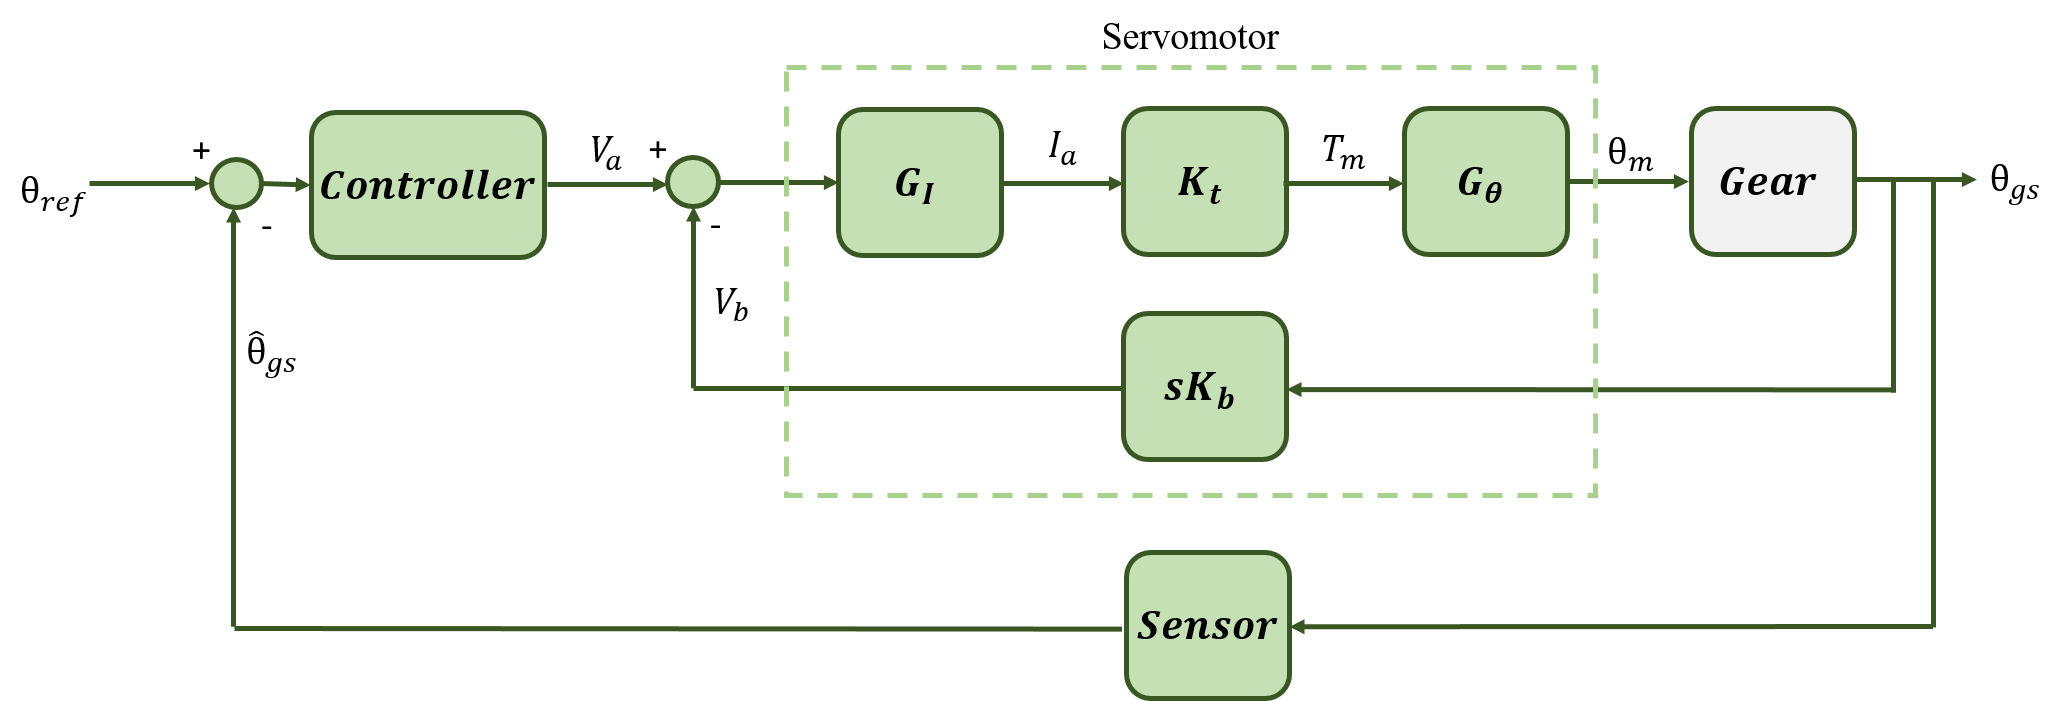
\includegraphics[scale=0.24]{../report/figures/servo+gear+noise+gear.png}
      \end{figure}  
  \end{block}
\end{frame}

%Sensor
\begin{frame}{Modelling}{Moving Angle System}
  \begin{block}{Moving Angle System:}

	  \begin{itemize}
	  	\item Sensor - measurement noise	  
	  \end{itemize}

	  \begin{figure}
        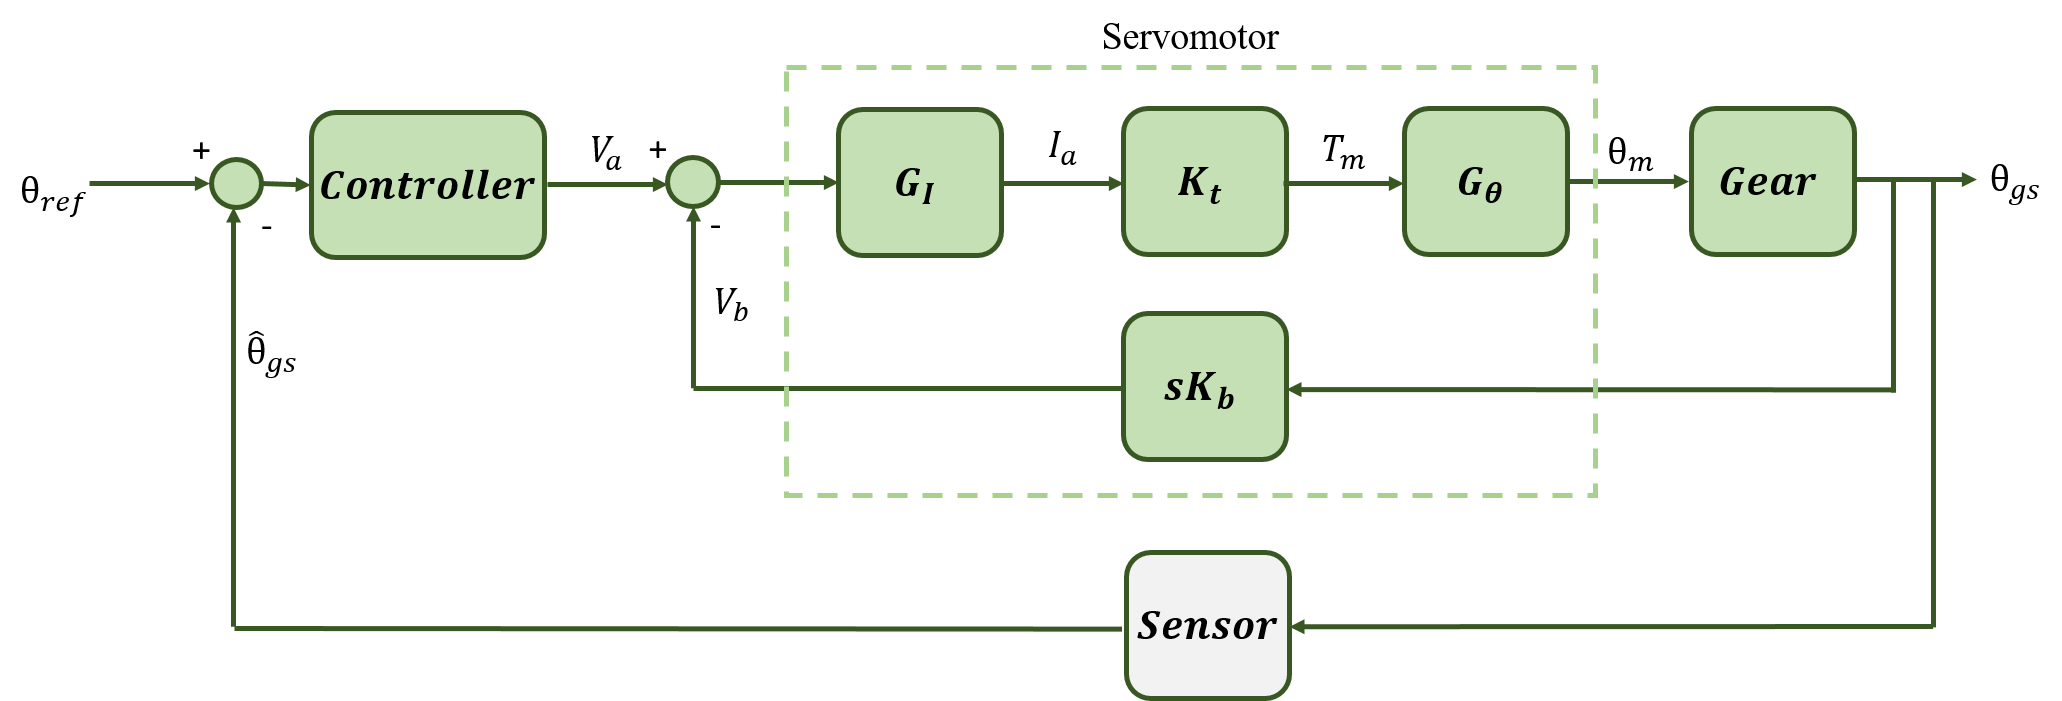
\includegraphics[scale=0.24]{../report/figures/servo+gear+noise+sensor.png}
      \end{figure}
  
  \end{block}
\end{frame}


%Controller
\begin{frame}{Modelling}{Moving Angle System}
  \begin{block}{Moving Angle System:}
	  \begin{itemize}
	  	\item Controller
	  \end{itemize}
	  \begin{figure}
        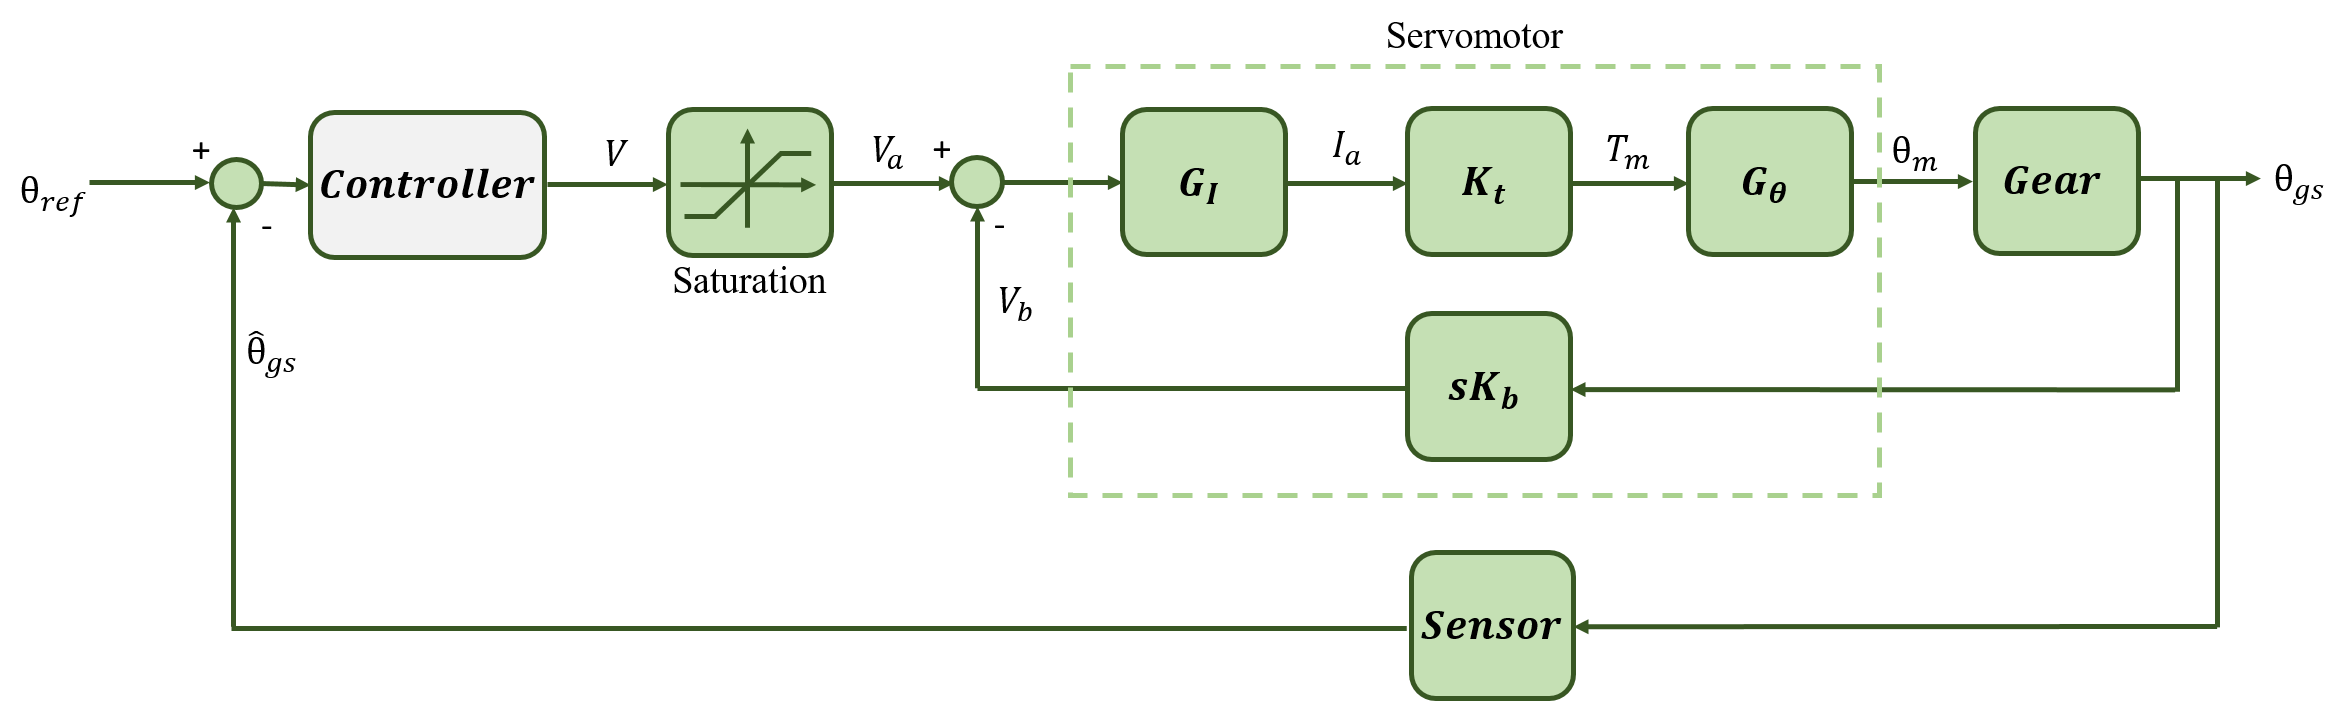
\includegraphics[scale=0.24]{../report/figures/servo+gear+noise+controller.png}
      \end{figure}
  \end{block}
\end{frame}

%Saturation
\begin{frame}{Modelling}{Moving Angle System}
  \begin{block}{Moving Angle System:}

	  \begin{itemize}
	  	\item Saturation - threshold set from -5V to 5V
	  \end{itemize}

	  \begin{figure}
        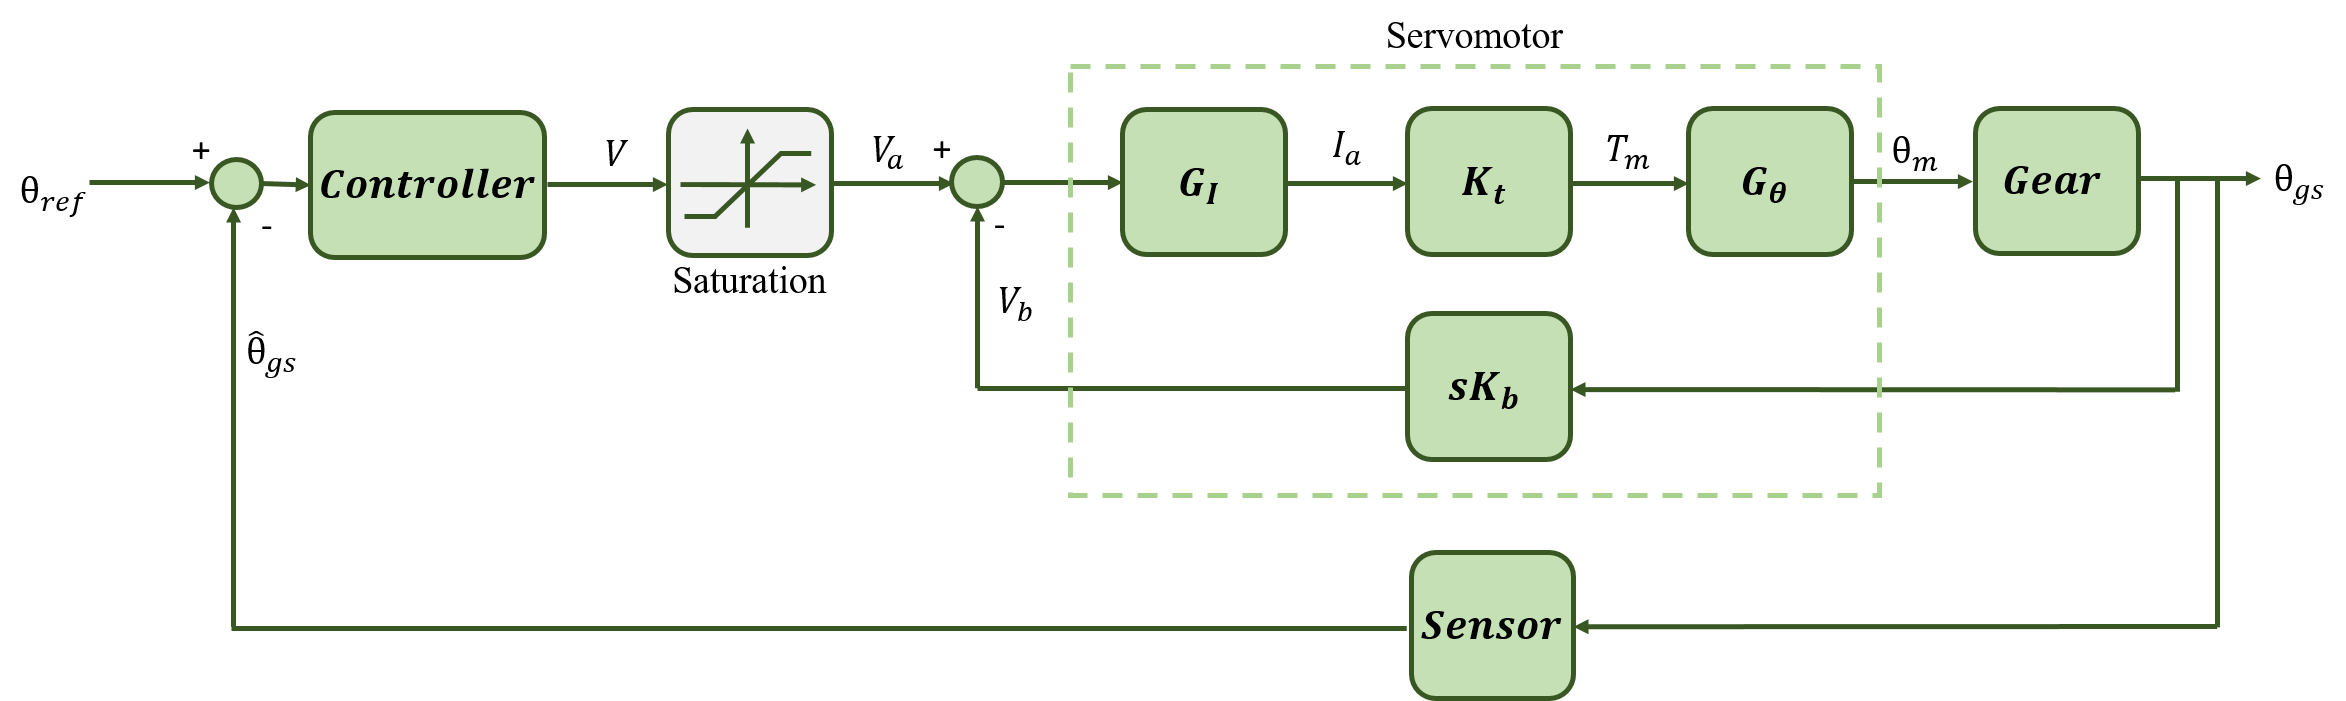
\includegraphics[scale=0.24]{../report/figures/servo+gear+noise+saturation.png}
      \end{figure}

  \end{block}
\end{frame}


%%%
%%Controller
\begin{frame}{Controller}{What controllers}
  \begin{block}{Type of control:}

	  \begin{itemize}
	  	\item PID control
	 	\begin{itemize}
	  	\item Proportional
	  	\item Derivative
	  	\item Integral
	  	\item Combination of them
	  \end{itemize}
	  \end{itemize}


  \end{block}
\end{frame}

%%%  HOW DID WE DESIGN THE CONTROLLERS?
%%Controller
\begin{frame}{Controller}{Tuning Method}
  \begin{block}{Good Gain Method:}
	  \begin{enumerate}
	  	\item Ti = $\infty$, Td = 0, Kp = 1
	  	\item Increase Kp until finding a slight overshoot
		\item Ti = 1.5$\cdot T_{out}$
		\item Td = $\frac{Ti}{4}$
	  \end{enumerate}
	  
  \end{block}
\end{frame}

%%Tuning Method
\begin{frame}{Controller}{Tuning Methods}
  \begin{block}{Good Gain Method}
  
	  \begin{enumerate}
	  	\item Ti = $\infty$, Td = 0, Kp = 1
	  \end{enumerate}
	  \begin{figure}
       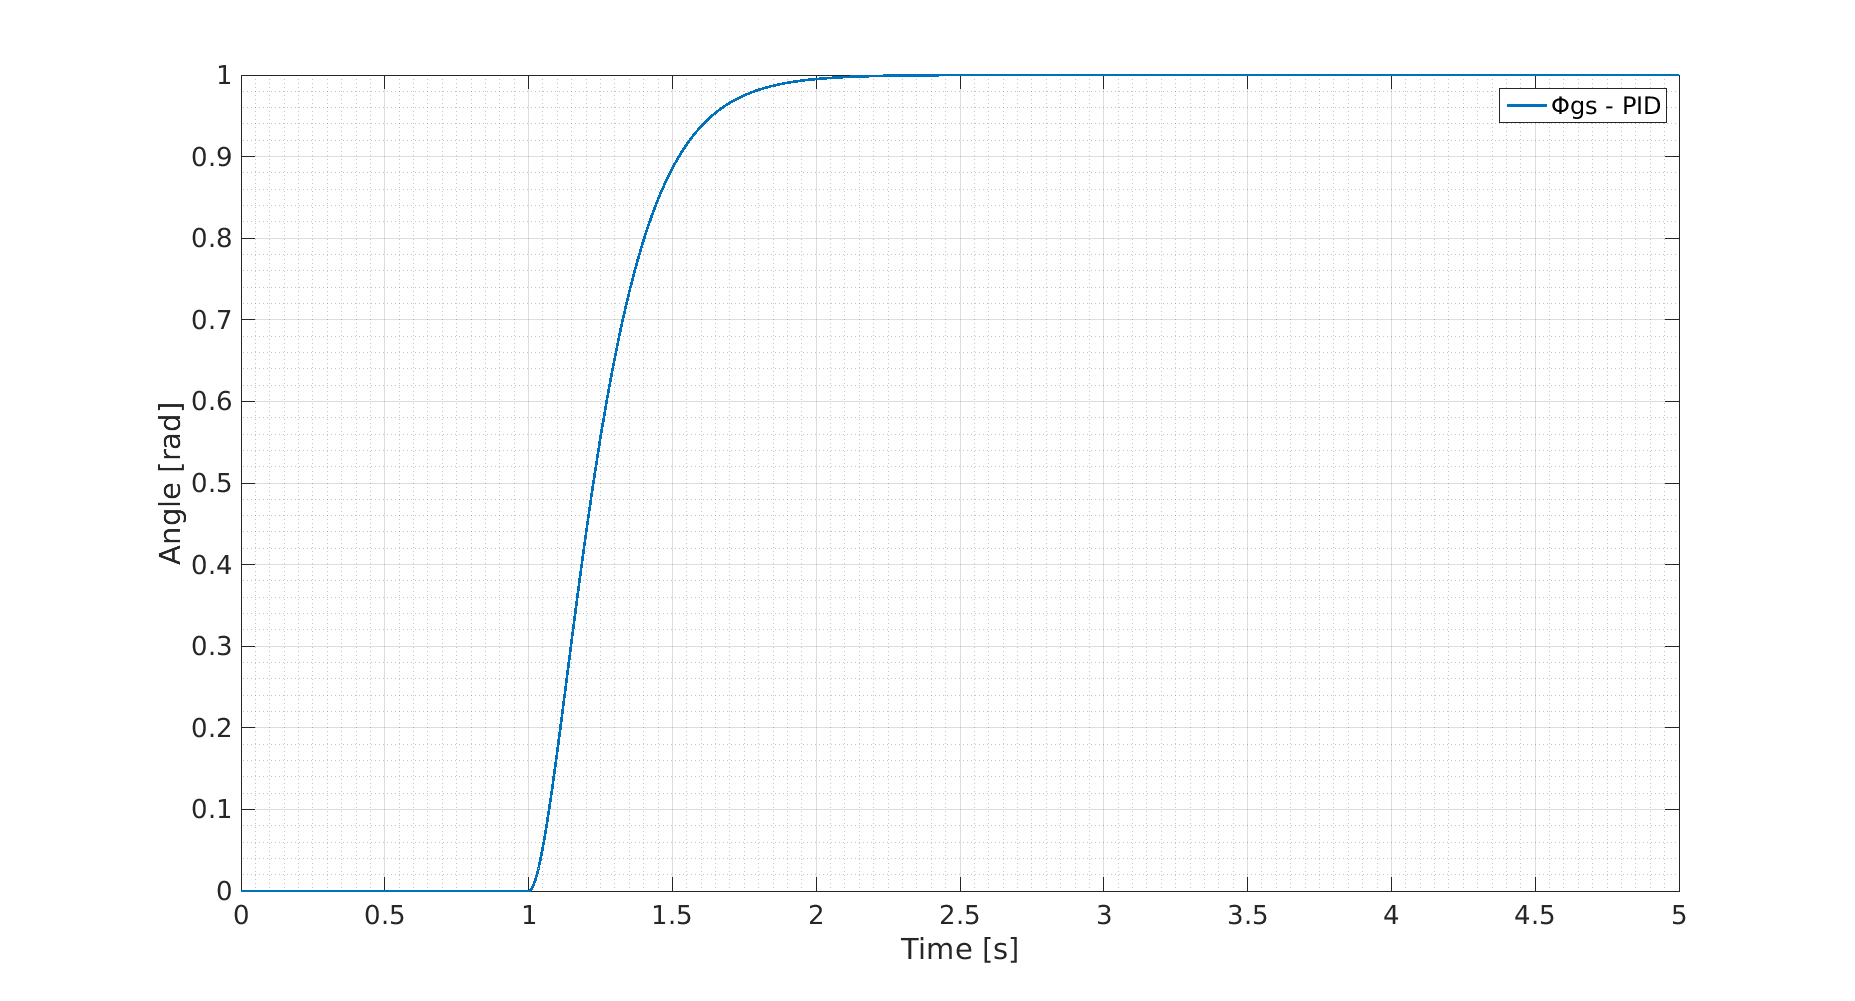
\includegraphics[scale=0.20]{../report/figures/GG1.png}
      \end{figure}
  
  \end{block}
\end{frame}

%Tuning Method
\begin{frame}{Controller}{Tuning Methods}
  \begin{block}{Good Gain Method}
  
	  \begin{enumerate}
	  \setcounter{enumi}{1}
	  	\item Increase Kp until finding a slight overshoot and well damped
	  	\begin{itemize}
	  	\item Save $T_{out}$ = Time between overshoot and undershoot
	  	\end{itemize}
	  \end{enumerate}
	  \begin{figure}
       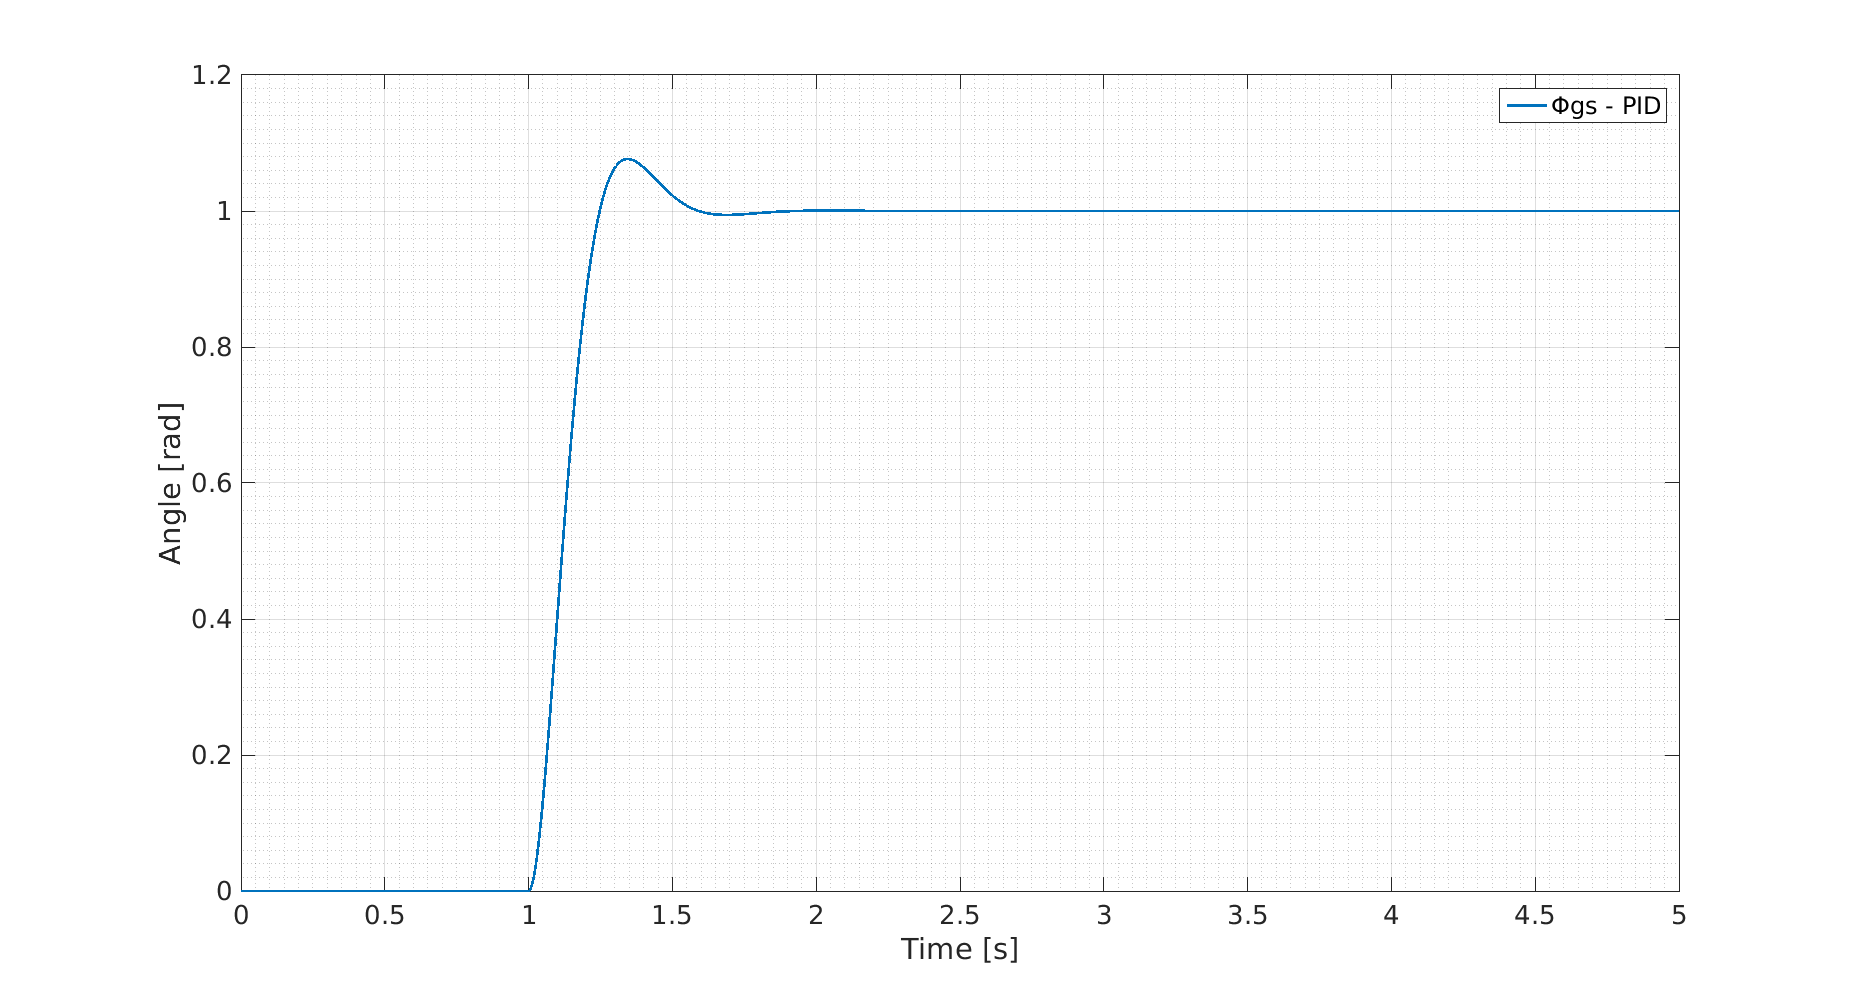
\includegraphics[scale=0.18]{../report/figures/GG2.png}
      \end{figure}
  
  \end{block}
\end{frame}

%Tuning Method
\begin{frame}{Controller}{Tuning Methods}
  \begin{block}{Good Gain Method}
  
	  \begin{enumerate}
	  \setcounter{enumi}{2}
	  	\item Ti = 1.5$\cdot T_{out}$
	  \end{enumerate}
	  \begin{figure}
       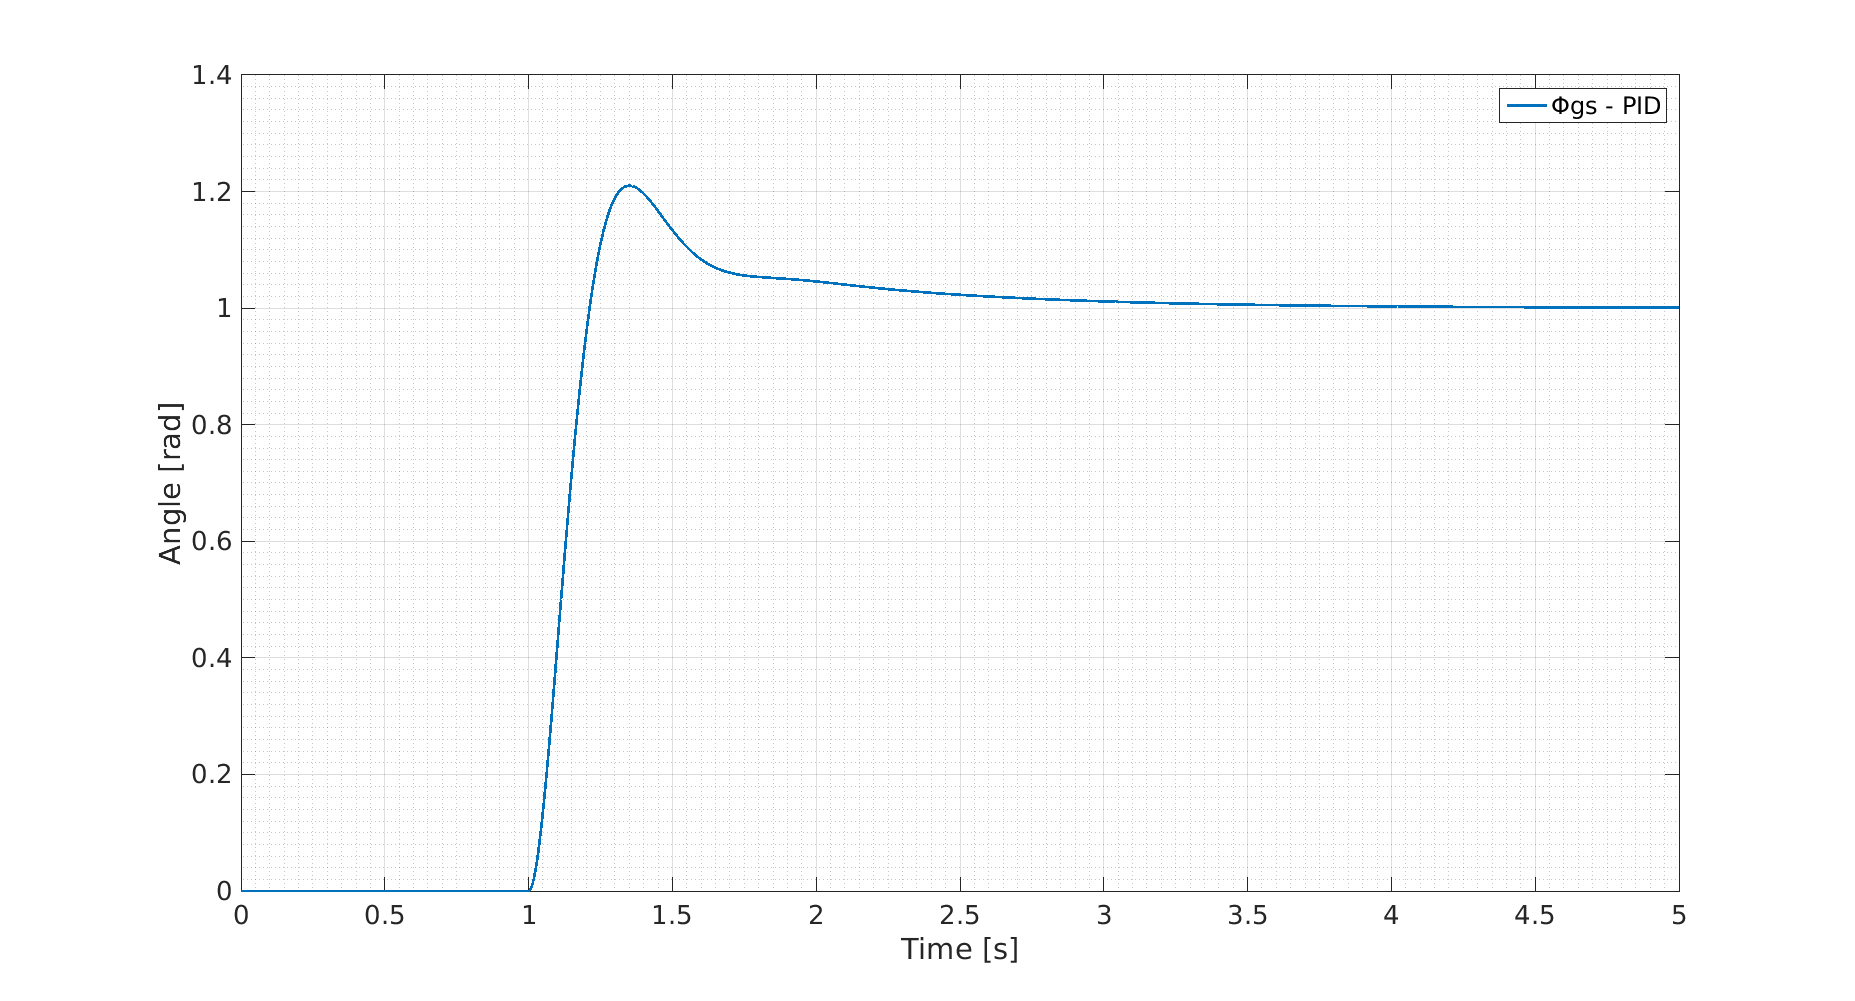
\includegraphics[scale=0.20]{../report/figures/GG3.png}
      \end{figure}
  
  \end{block}
\end{frame}



%Tuning Method
\begin{frame}{Controller}{Tuning Methods}
  \begin{block}{Good Gain Method}
  
	  \begin{enumerate}
	  \setcounter{enumi}{3}
	  	\item Td = $\frac{Ti}{4}$
	  \end{enumerate}
	  \begin{figure}
       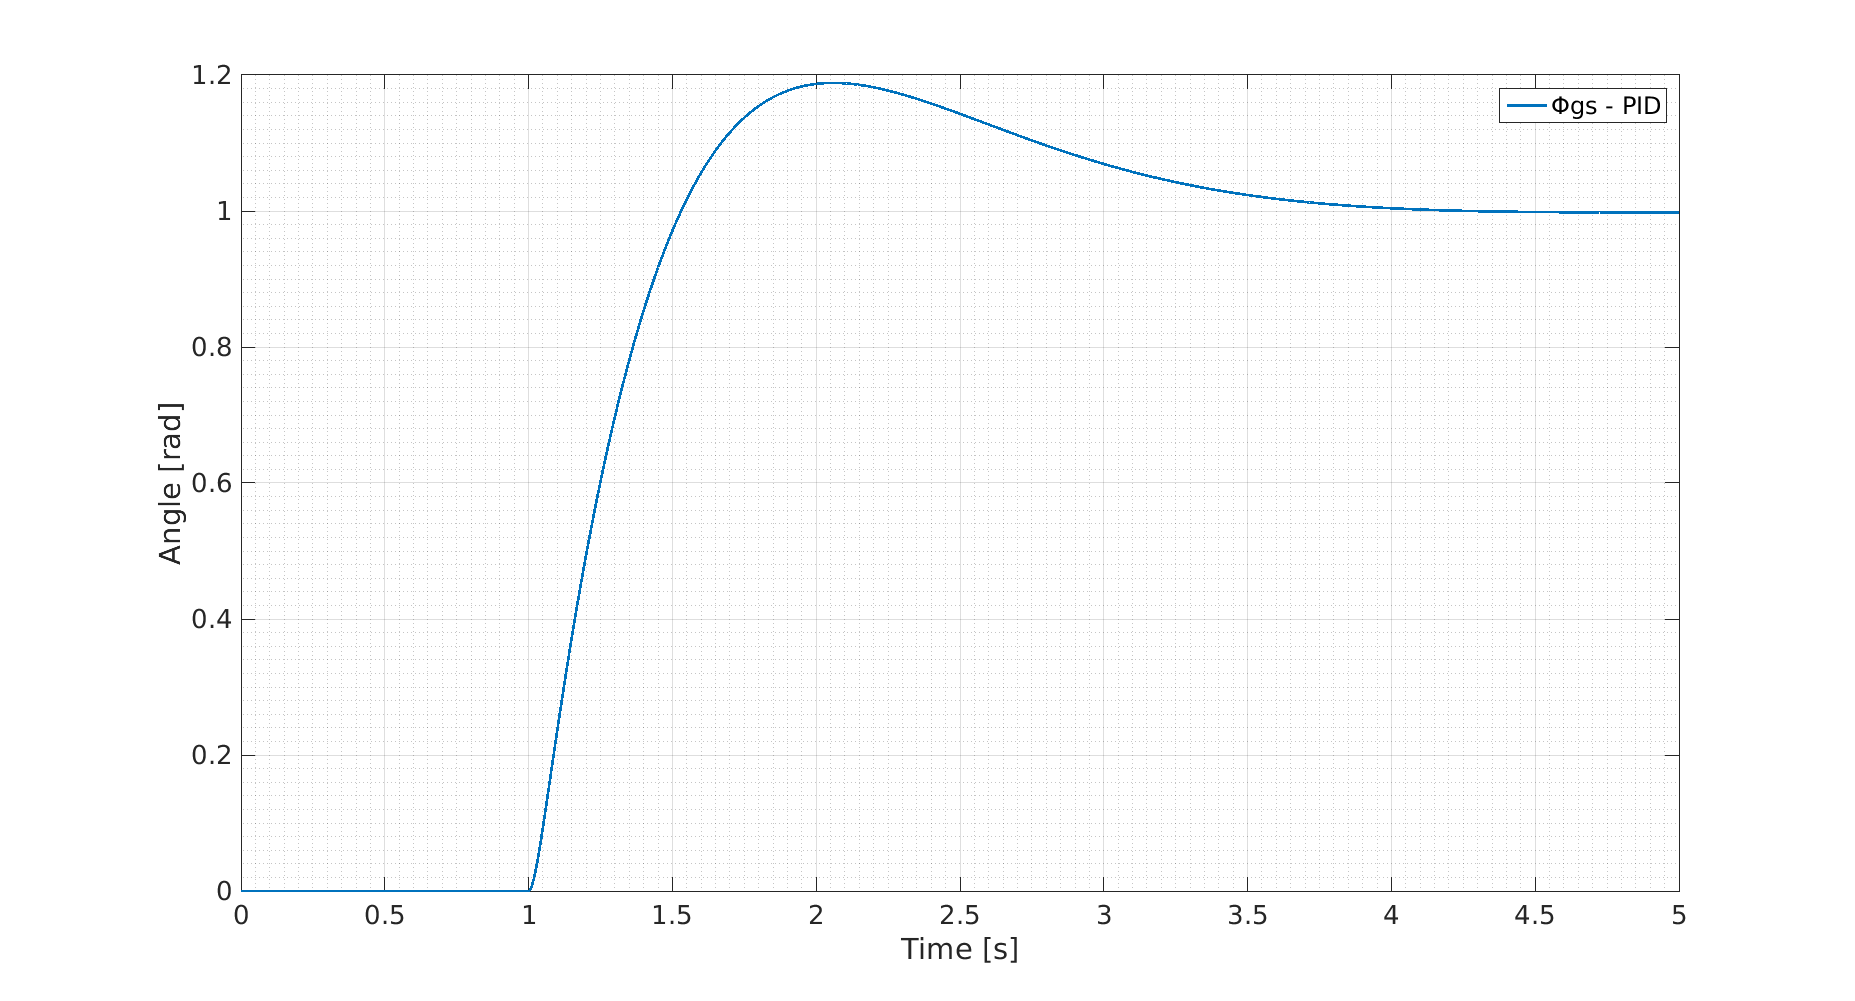
\includegraphics[scale=0.20]{../report/figures/GG4.png}
      \end{figure}
  
  \end{block}
\end{frame}


%Tuning Method
\begin{frame}{Controller}{Tuning Methods}
  \begin{block}{Good Gain Method}
  
	 \begin{itemize}
	  	\item Disadvantages:
	  \begin{itemize}
	  	\item Time consuming
	  	\item Uncertainties of the different steps	  	
	  \end{itemize}
	\end{itemize}
  
  \end{block}
\end{frame}


%%Controller
\begin{frame}{Controller}{Tuning method}
  \begin{block}{PID Simulink Box}

	  \begin{itemize}
	  \item Advantages:
	  \begin{itemize}
	  	\item Automatic Tuning Tool
	  	\item Design multiple controllers
	  	\item Adjust different parameters  	
	  \end{itemize}
	  \end{itemize}

  \end{block}
\end{frame}

%Comparison
\begin{frame}{Controller}{Comparison of step responses}
  \begin{block}{Different controllers:}
  
	  \begin{itemize}
	  	\item PI and PID - highest overshoot
	  		  \begin{itemize}
	  			\item 0.16rad and 0.19rad
	  			\item 9.17deg and 10.8deg
	  			\end{itemize}
	  	\item P and PD - no overshoot, shorter settling time, but still steady state error
	  \end{itemize}

	  \begin{figure}
        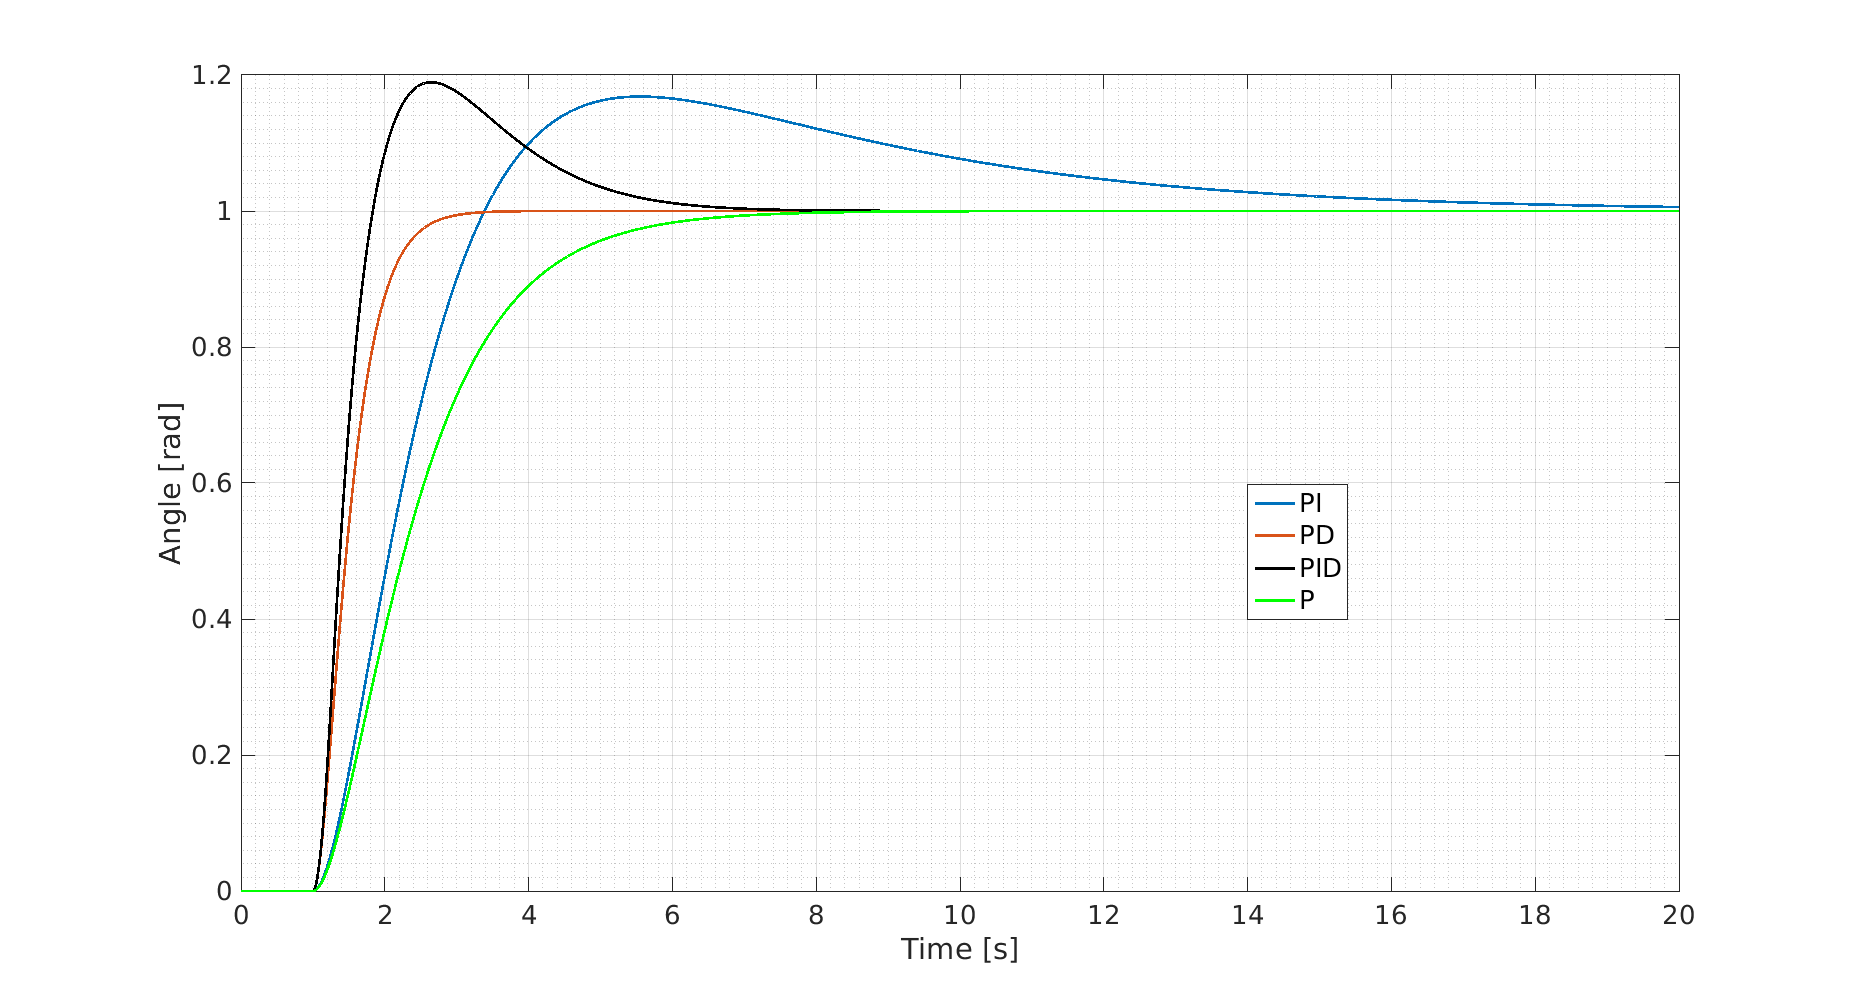
\includegraphics[scale=0.16]{../report/figures/full_comp.png}
      \end{figure}
  
  \end{block}
\end{frame}

%Comparison
\begin{frame}{Controller}{Comparison of step responses}
  \begin{block}{Different controllers with noise:}

	  \begin{itemize}
	  	\item PD faster than P
	  	\item PD reacts more to noise then P
	  \end{itemize}

	  \begin{figure}
        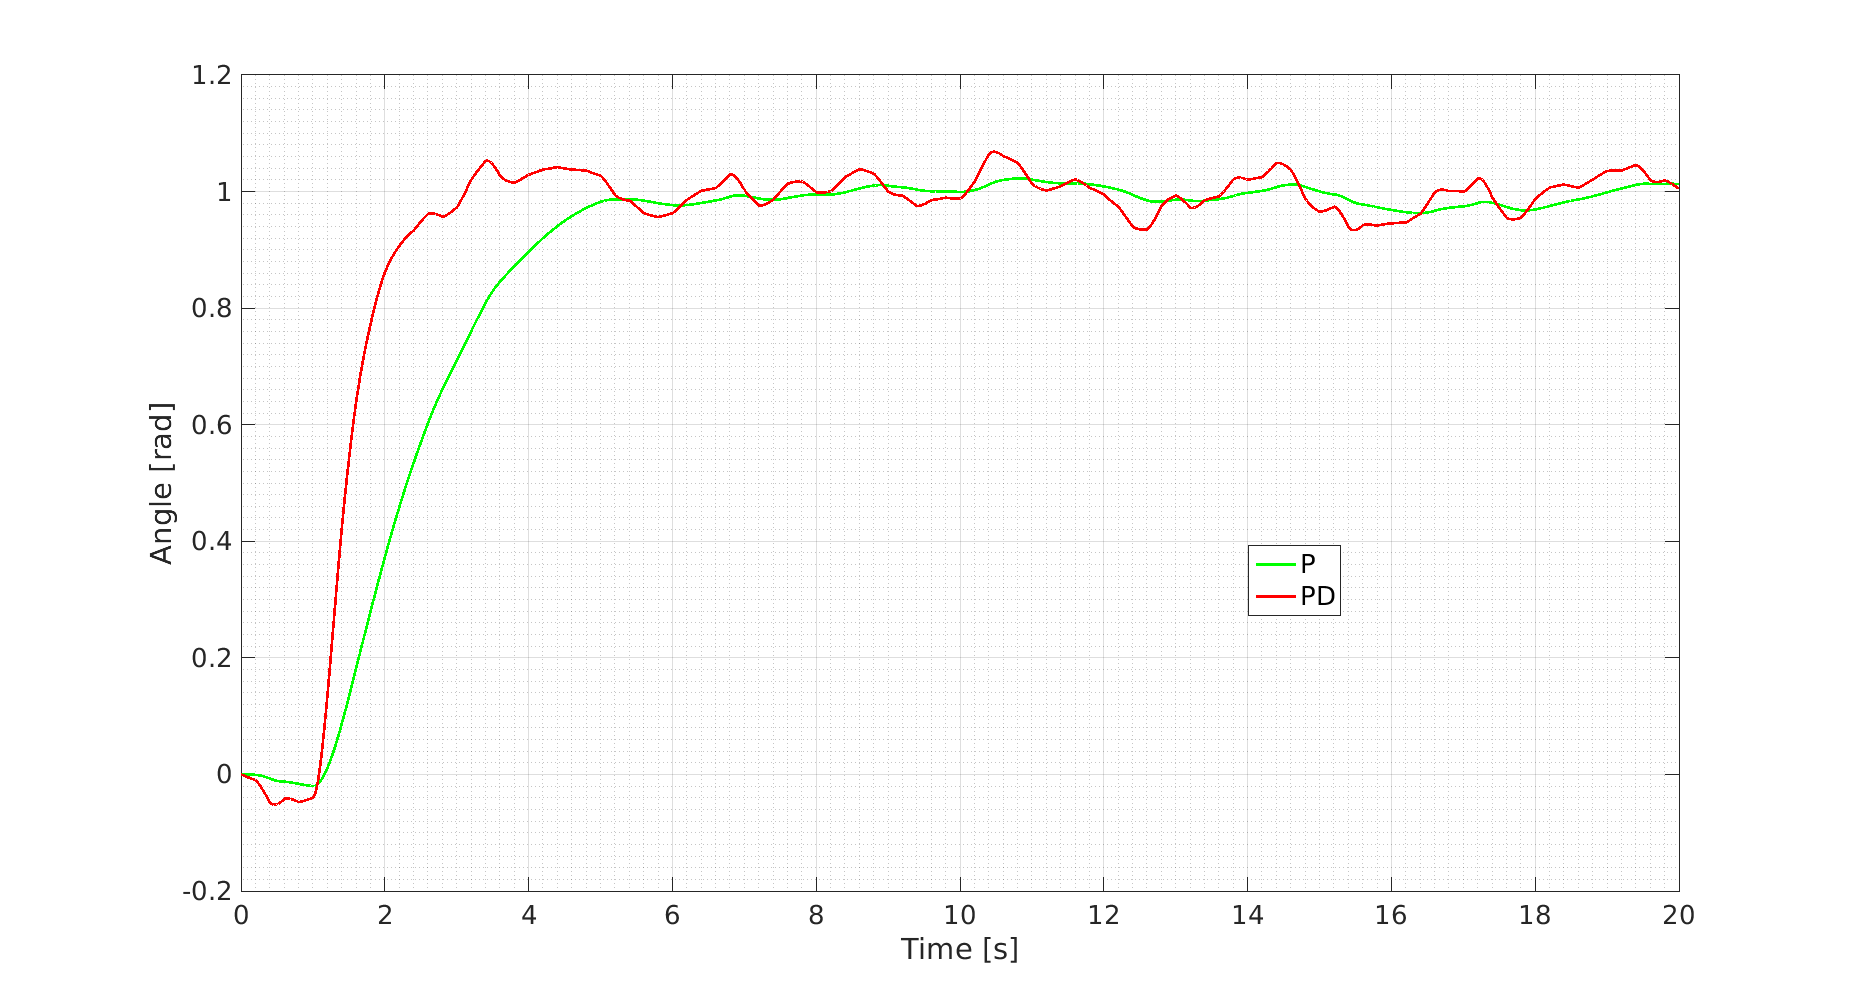
\includegraphics[scale=0.18]{../report/figures/PD_noise.png}
      \end{figure}
  
  \end{block}
\end{frame}

%%% CONTROLLER
%
%
%%Tuning Method
%\begin{frame}{Controller}{Tuning Methods}
%  \begin{block}{PID Simulink Box}
%
%
%	  \begin{itemize}
%	  	\item Weakness of Good Gain Method:
%	  		  \begin{itemize}
%	  	\item Time consuming
%	  	\item Uncertainties of the different steps
%	  \end{itemize}
%	  \item Advantages of PID Simulink Box
%	  \begin{itemize}
%	  	\item Automatic tuning tool
%	  	\item Include N term which avoids a "pure derivative" that reacts easily to noises
%	  \end{itemize}
%	  \end{itemize}
%  
%  \end{block}
%\end{frame}



%%Controller
%\begin{frame}{Controller}{Different controllers}
%  \begin{block}{Different controllers:}
%
%	  \begin{itemize}
%	  	\item PID control
%	 	\begin{itemize}
%	  	\item Proportional
%	  	\item Derivative
%	  	\item Integral
%	  	\item Combination of them
%	  \end{itemize}
%	  \end{itemize}
%
%
% 	  \begin{figure}
%        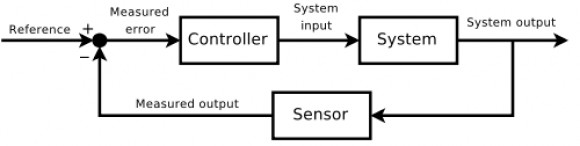
\includegraphics[scale=0.40]{../report/figures/control-theory-chart.jpg}
%      \end{figure} 
%  \end{block}
%\end{frame}
%%
%%Controller P
%\begin{frame}{Controller}{Different controllers}
%  \begin{block}{Proportional Term}
%
%	  \begin{itemize}
%	  	\item Output proportional to the error
%	  \end{itemize}
%
%	  \begin{figure}
%        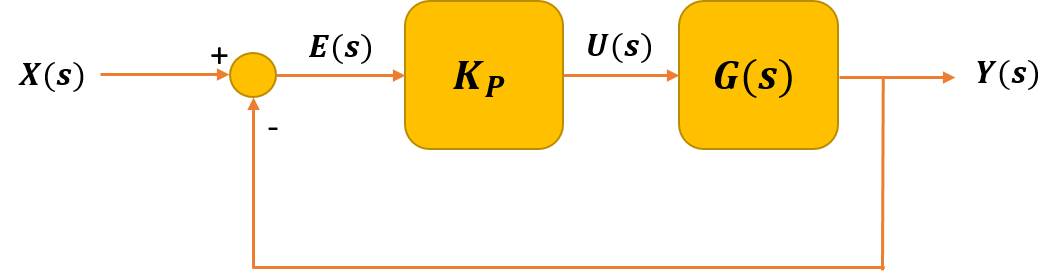
\includegraphics[scale=0.26]{../report/figures/propor_controller.png}
%      \end{figure}
%  
%  \end{block}
%\end{frame}

%%Controller I
%\begin{frame}{Controller}{Different controllers}
%  \begin{block}{Integral Term}
%
%	  \begin{itemize}
%	  	\item Sums the error term over time
%	  	\item No steady state error
%	  	\item Cause the present value to overshoot the reference value
%	  \end{itemize}
%
%	  \begin{figure}
%        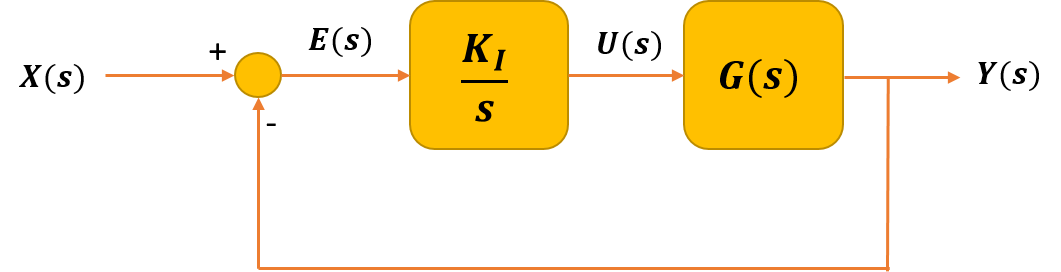
\includegraphics[scale=0.26]{../report/figures/integ_controller.png}
%      \end{figure}
%  
%  \end{block}
%\end{frame}

%%Controller D
%\begin{frame}{Controller}{Different controllers}
%  \begin{block}{Derivative Term}
%
%	  \begin{itemize}
%	  	\item Acts as a brake on the control effort
%	  	\item Highly sensitive to noise
%	  \end{itemize}
%
%	  \begin{figure}
%        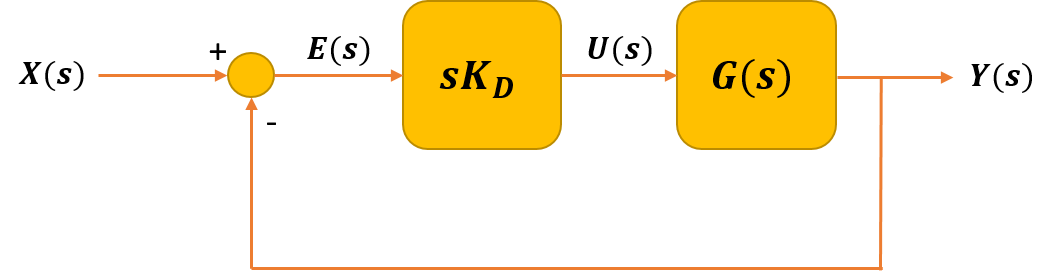
\includegraphics[scale=0.26]{../report/figures/deriv_controller.png}
%      \end{figure}
%  
%  \end{block}
%\end{frame}

%%Controller PI
%\begin{frame}{Controller}{Different controllers}
%  \begin{block}{PI Controller}
%
%	  \begin{itemize}
%	  	\item Eliminate the steady state error
%	  	\item Negative impact on the speed of the response
%	  	\item Should be applied when speed is not an important parameter
%	  \end{itemize}
%
%	  \begin{figure}
%        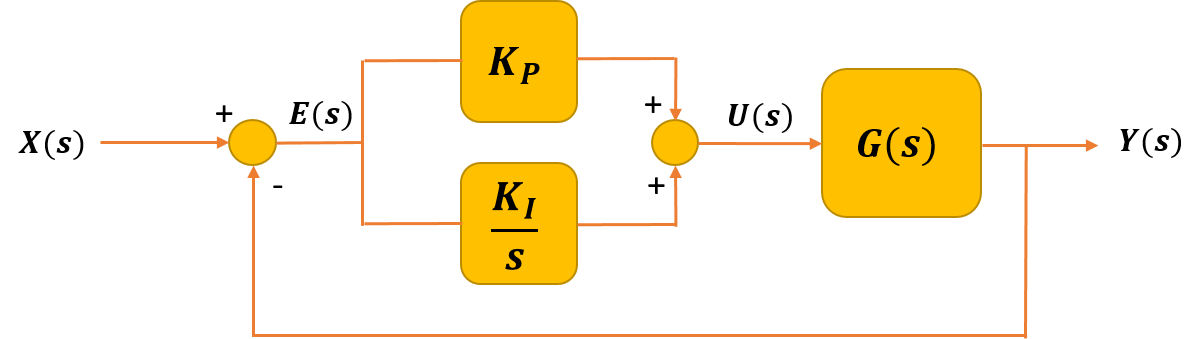
\includegraphics[scale=0.26]{../report/figures/PI_controller.png}
%      \end{figure}
%  
%  \end{block}
%\end{frame}
%
%
%%Controller PD
%\begin{frame}{Controller}{Different controllers}
%  \begin{block}{PD Controller}
%
%	  \begin{itemize}
%	  	\item Why is PD alone good?
%	  \end{itemize}
%
%	  \begin{figure}
%        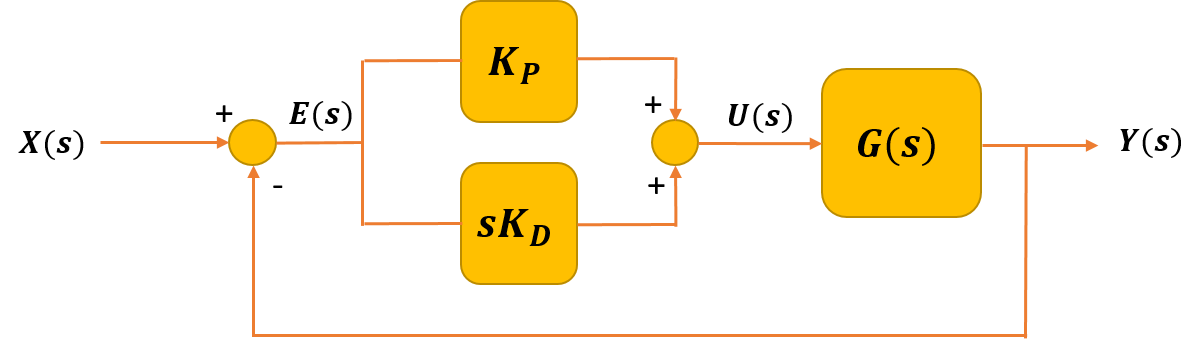
\includegraphics[scale=0.26]{../report/figures/PD_controller.png}
%      \end{figure}
%  
%  \end{block}
%\end{frame}
%
%%Controller PID
%\begin{frame}{Controller}{Different controllers}
%  \begin{block}{PID Controller}
%
%	  \begin{itemize}
%	  	\item Eliminate steady state error
%	  	\item Fast response
%	  	\item Higher stability
%	  	\item (Derivative Term) Reduction of the overshoot and oscillations
%	  \end{itemize}
%
%	  \begin{figure}
%        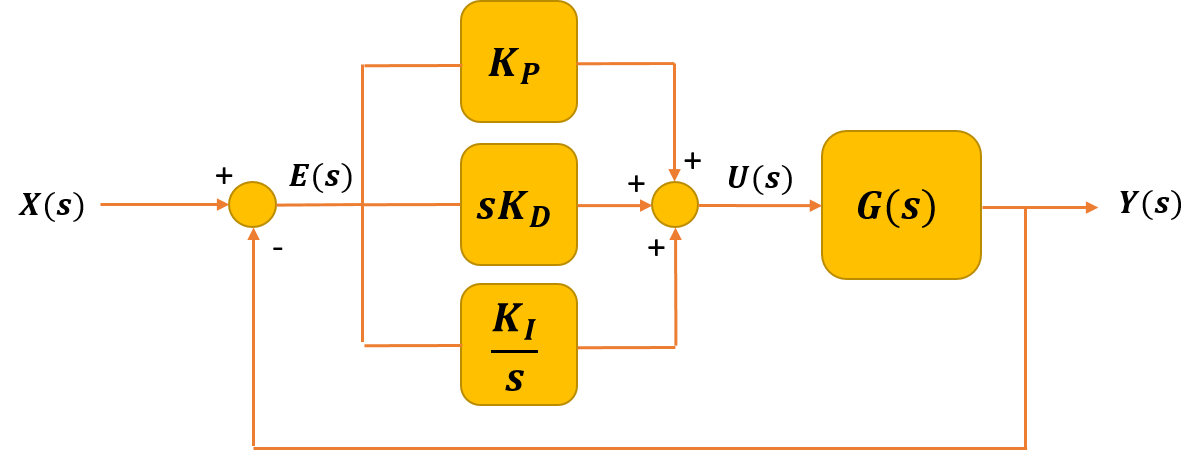
\includegraphics[scale=0.26]{../report/figures/PID_controller.png}
%      \end{figure}
%  
%  \end{block}
%\end{frame}





\subsection{Simulation}

\begin{frame}{Simulation}{LOS Coverage Map}
  \begin{block}{Parameters taken into account for map simulation:}

	  \begin{itemize}
	  	\item Terrain elevation
	  	\item Curvature of the Earth
	  	\item Altitude of UA and GS
	  \end{itemize}

	  \begin{figure}
        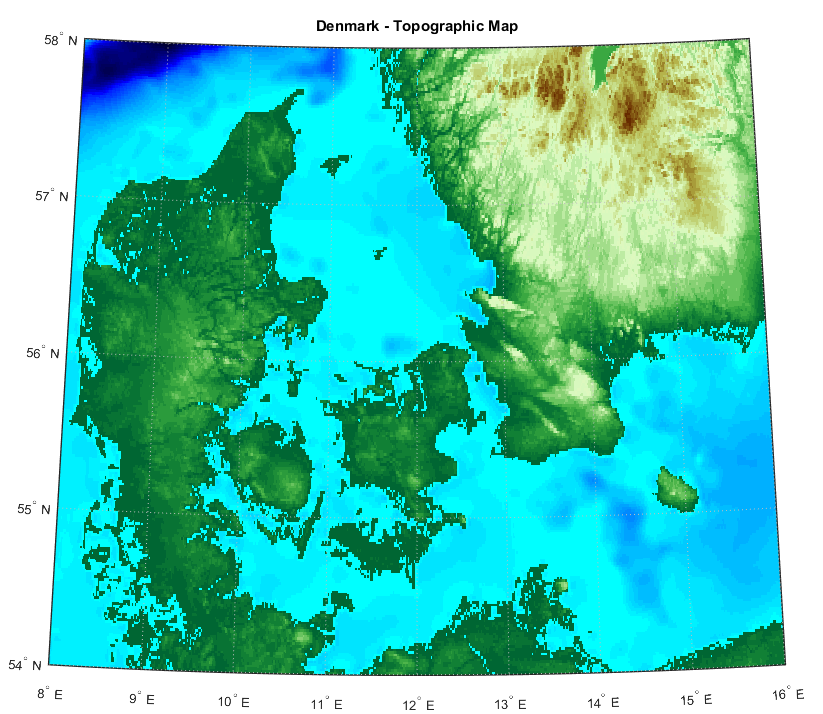
\includegraphics[scale=0.26]{../report/figures/dk_map.png}
      \end{figure}
  
  \end{block}
\end{frame}

\begin{frame}{Simulation}{LOS Coverage Map}
  \begin{block}{Working Principle}
	  \begin{itemize}
	  	\item Import topography map
	  	\item Input GS and UA altitude
	  	\item Choose GS and UA locations on map to plot LOS distance
	  	\item Choose GS location on map to plot LOS coverage map
	  \end{itemize}
  \end{block}
\end{frame}

\begin{frame}{Simulation}{LOS between UA and GS} 
  	\begin{figure}
        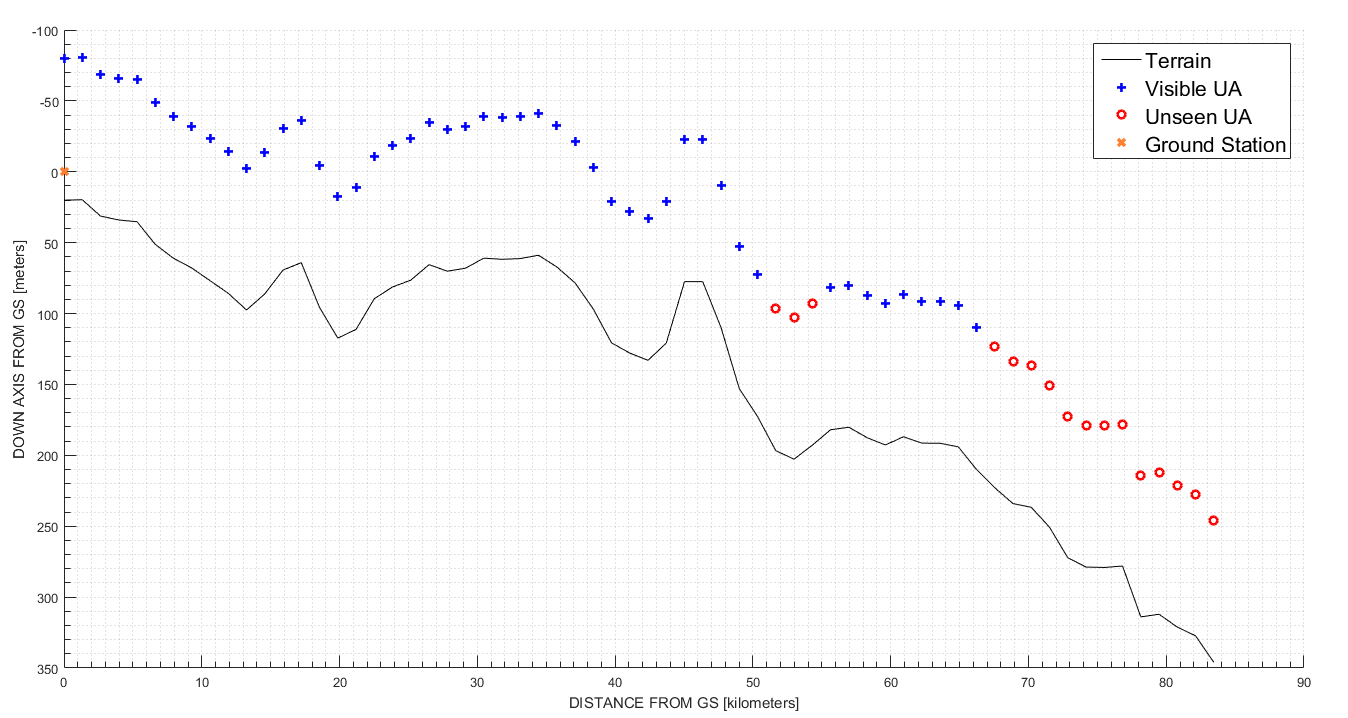
\includegraphics[scale=0.29]{../report/figures/los_2points.png}
    \end{figure}
\end{frame}

\begin{frame}{Simulation}{LOS Coverage Map} 
  	\begin{figure}
        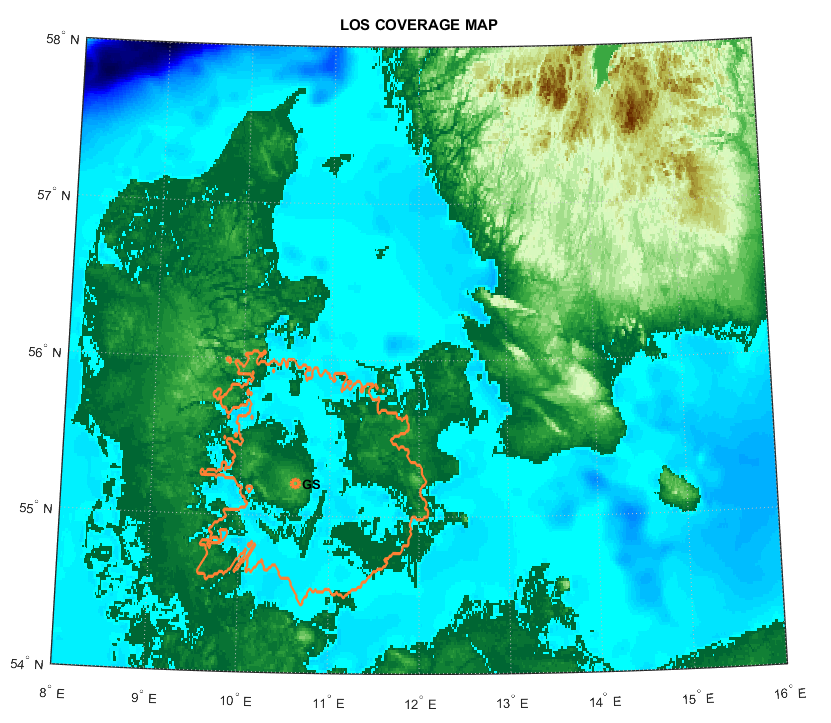
\includegraphics[scale=0.40]{../report/figures/los_odense.png}
    \end{figure}
\end{frame}

\begin{frame}{Simulation}{2D UAS}
	\begin{block}{2D UAS Block Diagram}
		\begin{itemize}
		  	\item Cartesian system (Simplistic)
		  	\item 1 DoF - azimuth angle ($\theta$)
		  	\item Compute optimal azimuth angle for UA and GS 
		\end{itemize}

		\begin{figure}
	        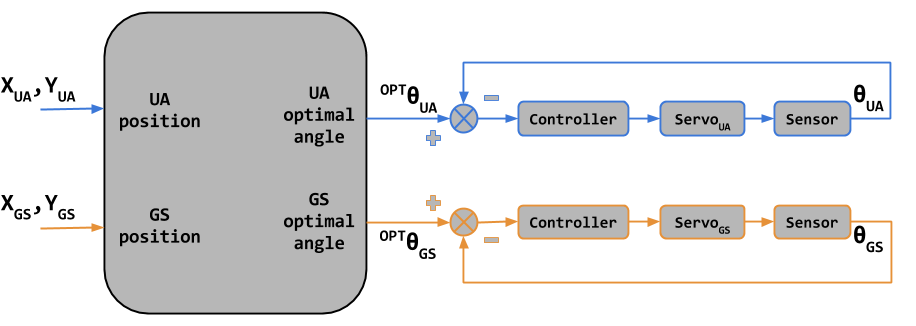
\includegraphics[scale=0.32]{figures/2D_system.png}
	    \end{figure}
    \end{block}
\end{frame}

\begin{frame}{Simulation}{3D UAS}
  \begin{block}{3D UAS Block Diagram}
	\begin{itemize}
	  	\item Realistic Earth Model - WGS84
	  	\item Curvature of the Earth
	  	\item Relief of Earth's surface 
	  	\item Real GPS position: latitude, longitude and altitude
	\end{itemize}

	\begin{figure}
		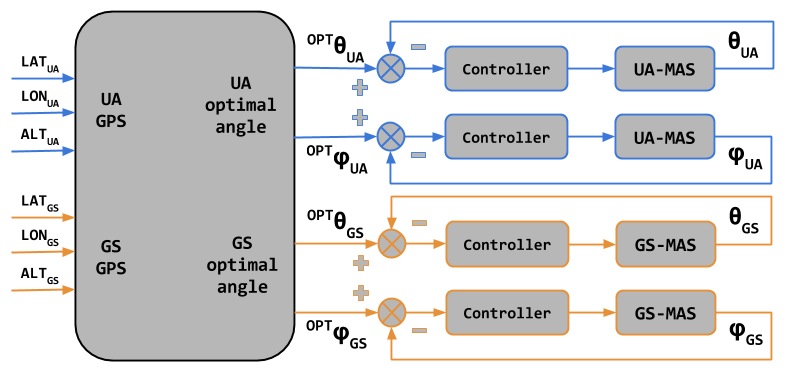
\includegraphics[scale=0.33]{figures/3D_system.png}
	\end{figure}
  \end{block}
\end{frame}



\section{Results}
\subsection{Results}

\begin{frame}{Results}{}
  \begin{itemize}
    \item<1-> There are probably still a lot of bugs in the theme. If you should find one, then please let me know. No bug is too small!
    \item<2-> Also, please contact me, if you have some exciting new ideas or just some simple usability improvements.
  \end{itemize}
\end{frame}
\begin{frame}{Results}{Angle Range}

  \begin{block}{Goal}
	Describing the movement of the antennas when the UA is flying far away from the GS. 
  \end{block}

  \begin{figure}[H]
    \centerline{
    \subfigure[UAS Map]
    $\vcenter{\hbox{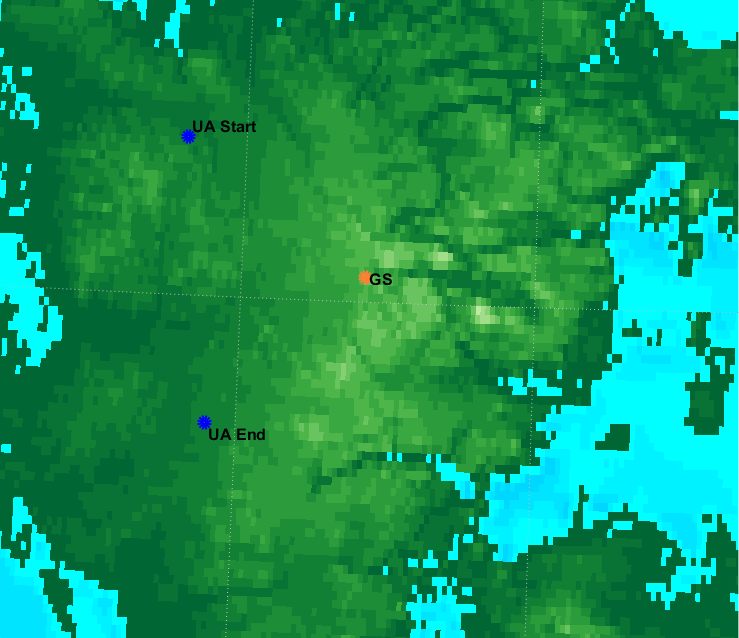
\includegraphics[scale=0.3]{figures/s1_zoom.png}}}$
    \subfigure[Distance between UA and GS]
    $\vcenter{\hbox{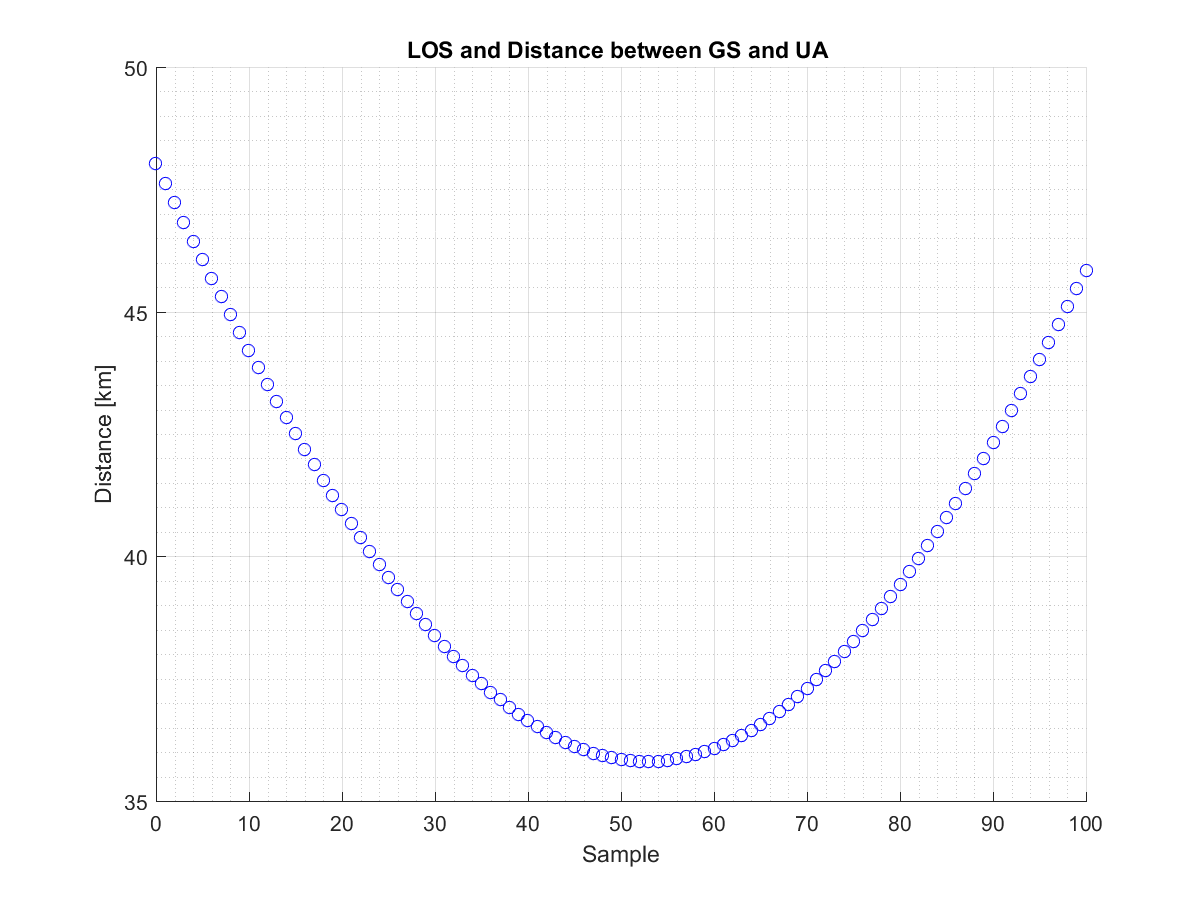
\includegraphics[scale=0.31]{figures/s1_los.png}}}}$
  \end{figure}

\end{frame}



\begin{frame}{Results}{Angle Range}

  \begin{block}{GS Tracking Angles}  
  
  \begin{figure}[H]
    \centerline{
    \subfigure[UAS Map]{
    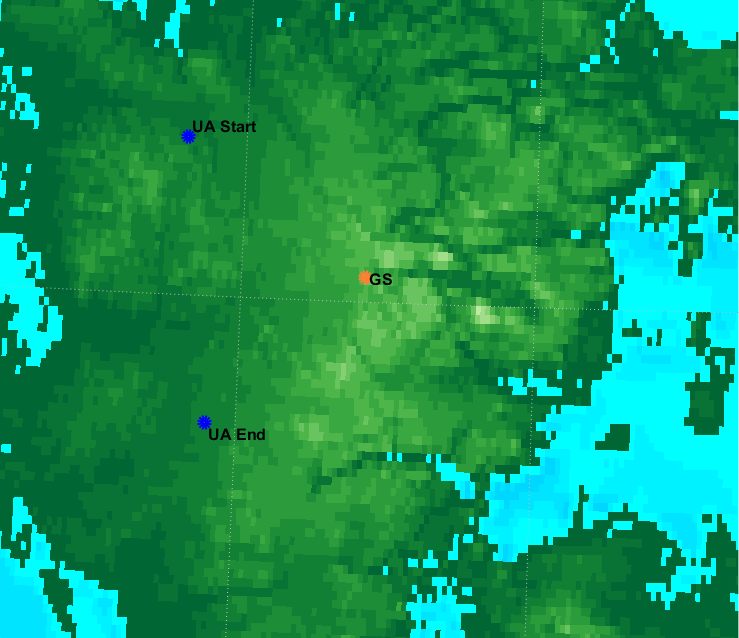
\includegraphics[scale=0.25]{figures/s1_zoom.png}}
    \subfigure[Distance between UA and GS]{
    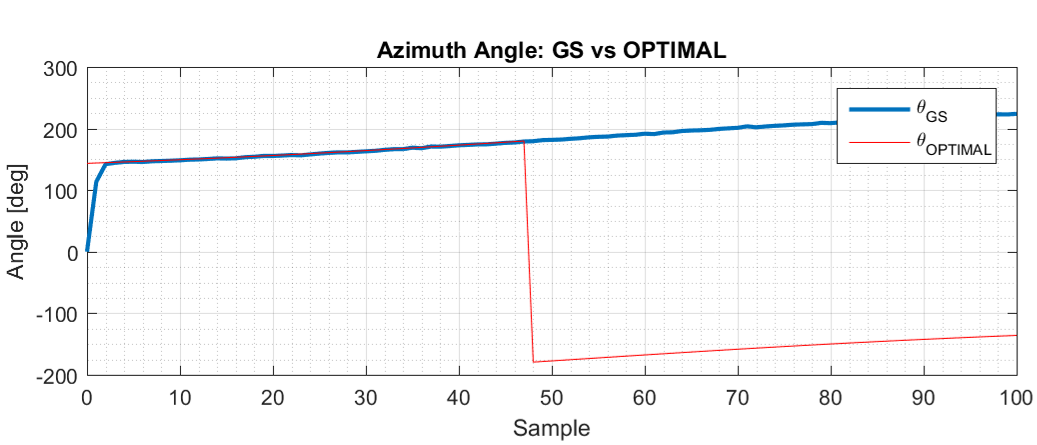
\includegraphics[scale=0.35]{figures/s1_pd_gs.png}}}
  \end{figure}
  
  \end{block}

\end{frame}
\subsection{Scenario 2}

\begin{frame}{Results}{Scenario 2 - Curvature of the Earth}

  \begin{block}{Goal}
	Describing the movement of the antennas when the UA is flying in a straight towards a further position.
	Show that the curvature of the Earth is taken into account.
  \end{block}

  \begin{figure}[H]
    \centerline{
    \subfigure[UAS Map]{
    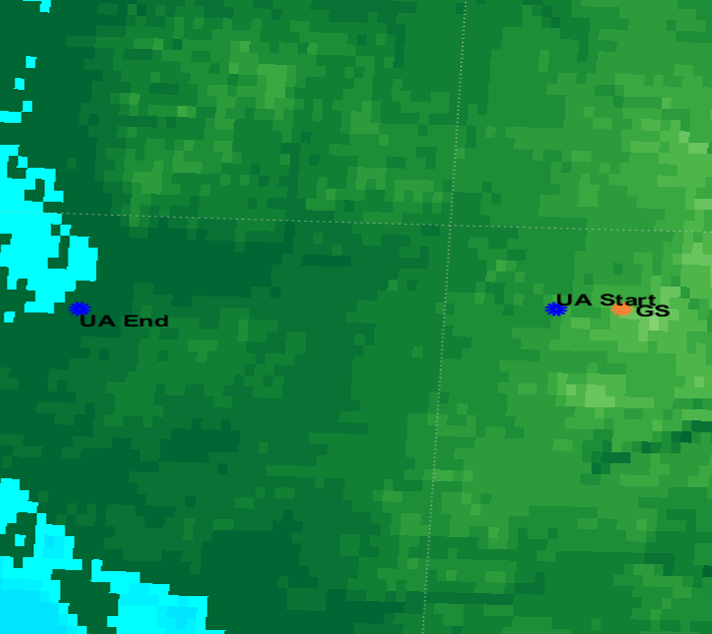
\includegraphics[scale=0.25]{figures/s2_zoom.png}}
    \hfill
    \subfigure[Distance between UA and GS]{
    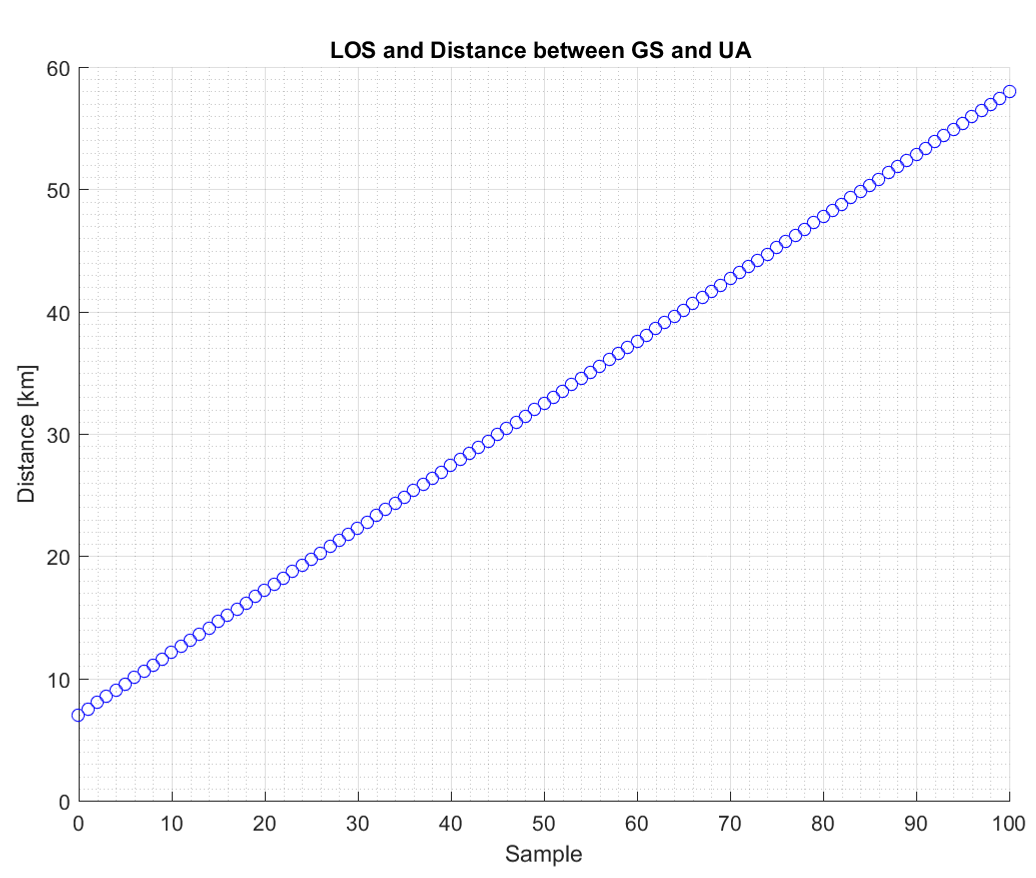
\includegraphics[scale=0.35]{figures/s2_los.png}}}
  \end{figure}

\end{frame}



\begin{frame}{Results}{Scenario 2 - Curvature of the Earth}

  \begin{block}{GS Tracking Angles}  
  
  \begin{figure}[H]
    \centerline{
    \subfigure[UAS Map]{
    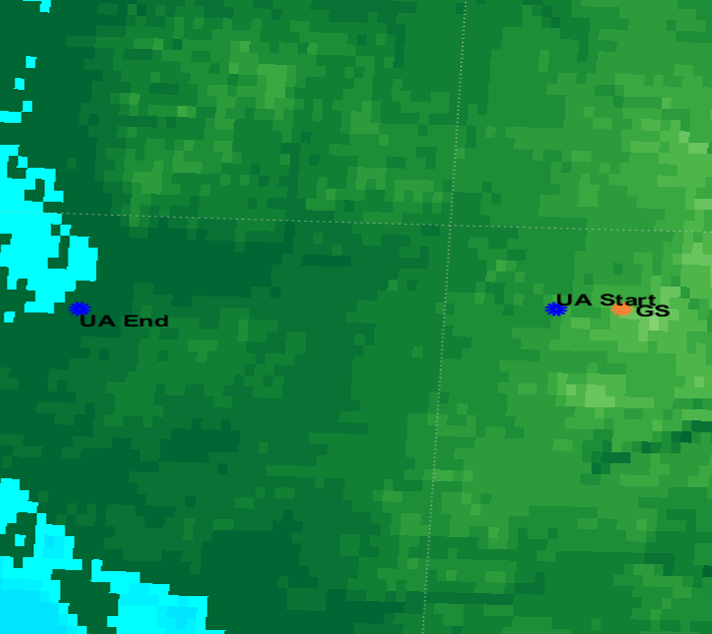
\includegraphics[scale=0.25]{figures/s2_zoom.png}}
    \hfill
    \subfigure[Azimuth and elevation angles of the antenna on the GS]{
    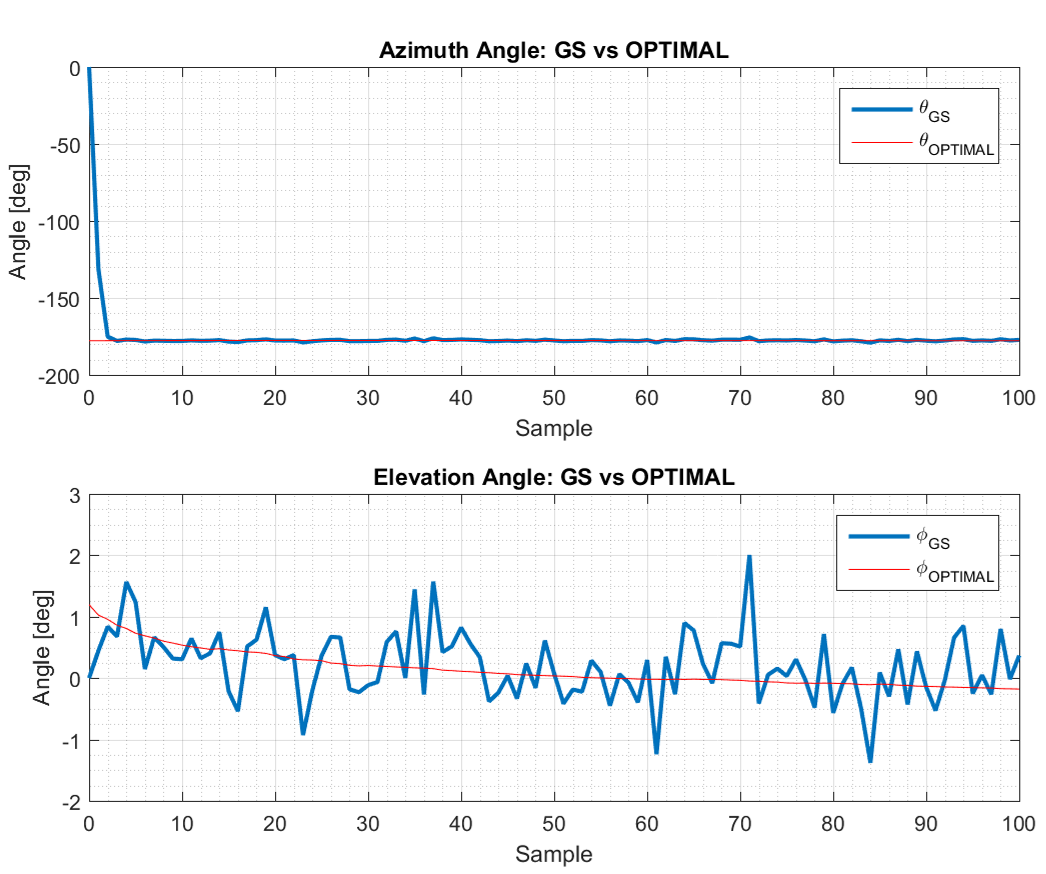
\includegraphics[scale=0.35]{figures/s2_gs.png}}}
  \end{figure}
  
  \end{block}

\end{frame}



\begin{frame}{Results}{Scenario 2 - Curvature of the Earth}

  \begin{block}{UA Tracking Angles}  
  
  \begin{figure}[H]
    \centerline{
    \subfigure[UAS Map]{
    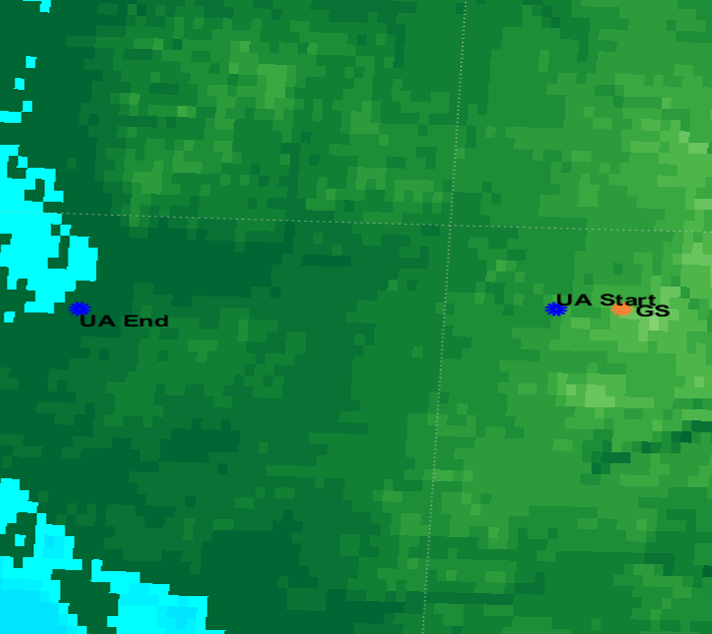
\includegraphics[scale=0.25]{figures/s2_zoom.png}}
    \hfill
    \subfigure[Azimuth and elevation angles of the antenna on the UA]{
    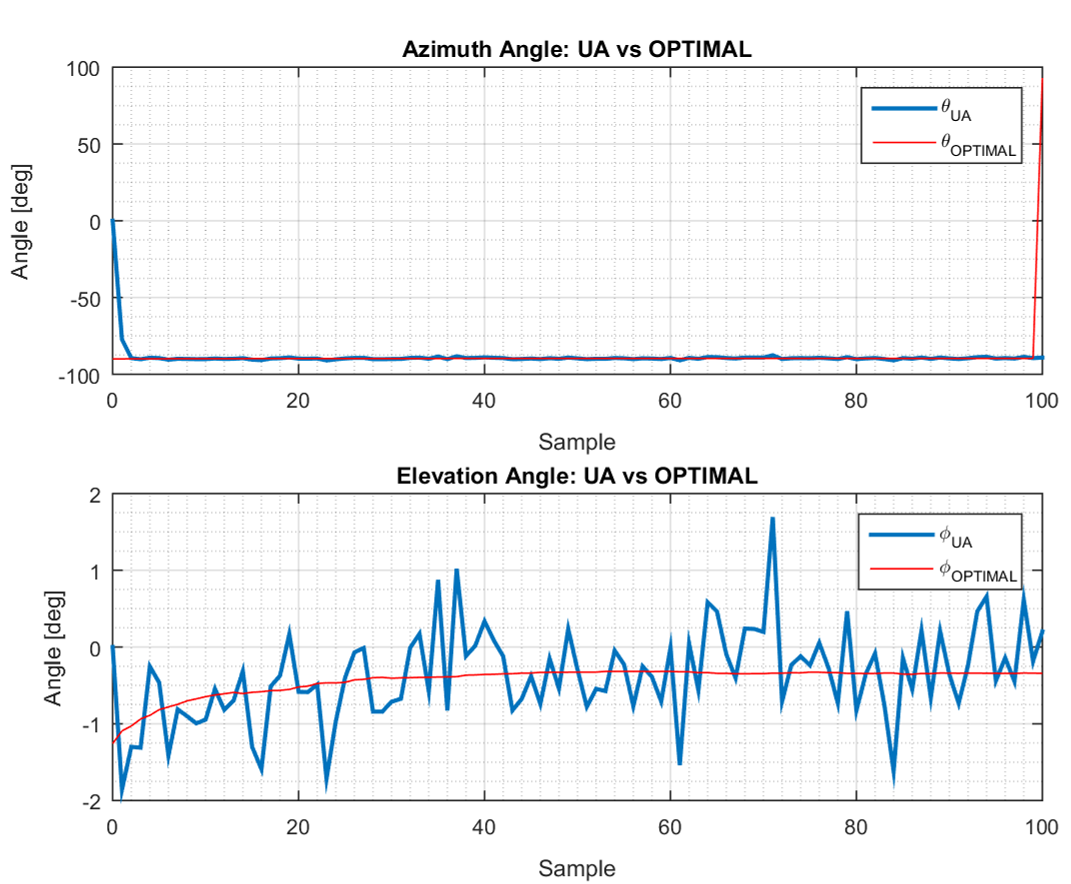
\includegraphics[scale=0.35]{figures/s2_ua.png}}}
  \end{figure}
  
  \end{block}

\end{frame}



\begin{frame}{Results}{Scenario 2 - Curvature of the Earth}

  \begin{block}{Signal Power}  
  
  \begin{figure}[H]
    \centerline{
    \subfigure[UAS Map]{
    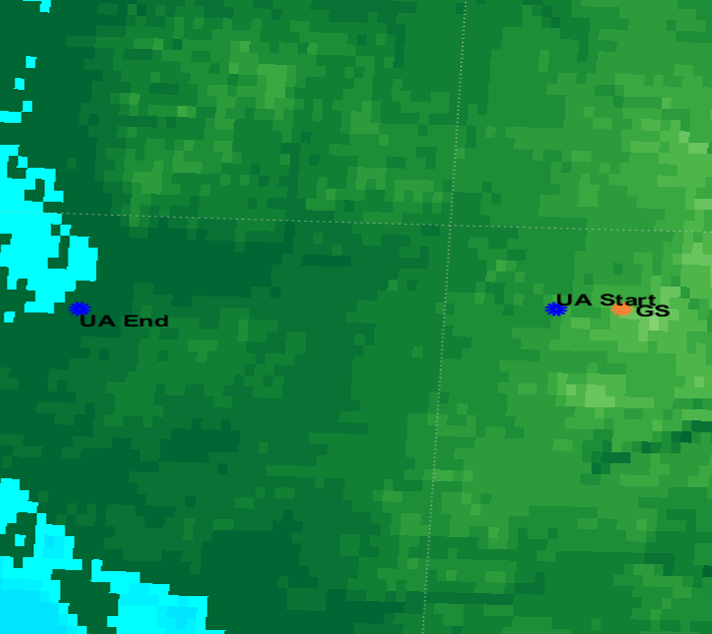
\includegraphics[scale=0.25]{figures/s2_zoom.png}}
    \hfill
    \subfigure[Power at the receiver]{
    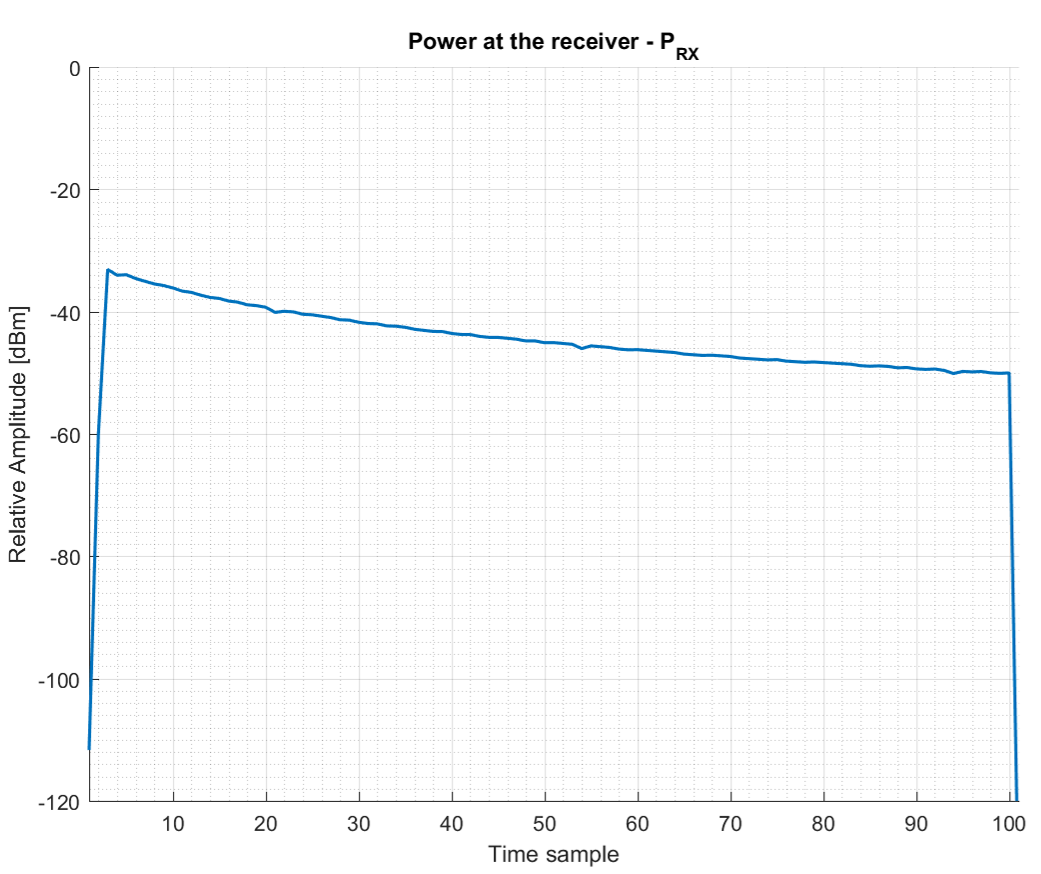
\includegraphics[scale=0.35]{figures/s2_power.png}}}
  \end{figure}
  
  \end{block}

\end{frame}

\subsection{Scenario 3}

\begin{frame}{Results}{Scenario 3 - Above the GS}

  \begin{block}{Goal}
	Describe the movement of the antennas when the UA is flying above the GS.
  \end{block}

  \begin{figure}[H]
    \centerline{
    \subfigure[UAS Map]{
    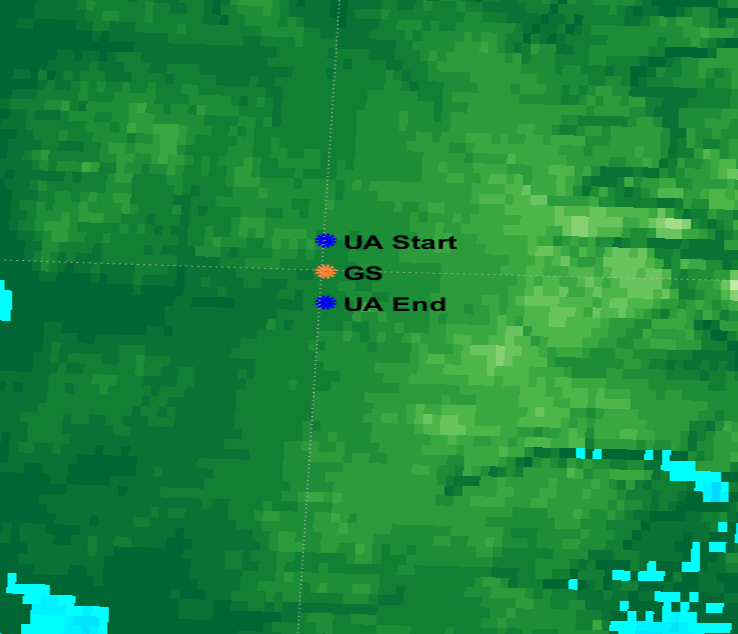
\includegraphics[scale=0.25]{figures/s3_zoom.png}}
    \hfill
    \subfigure[Distance between UA and GS]{
    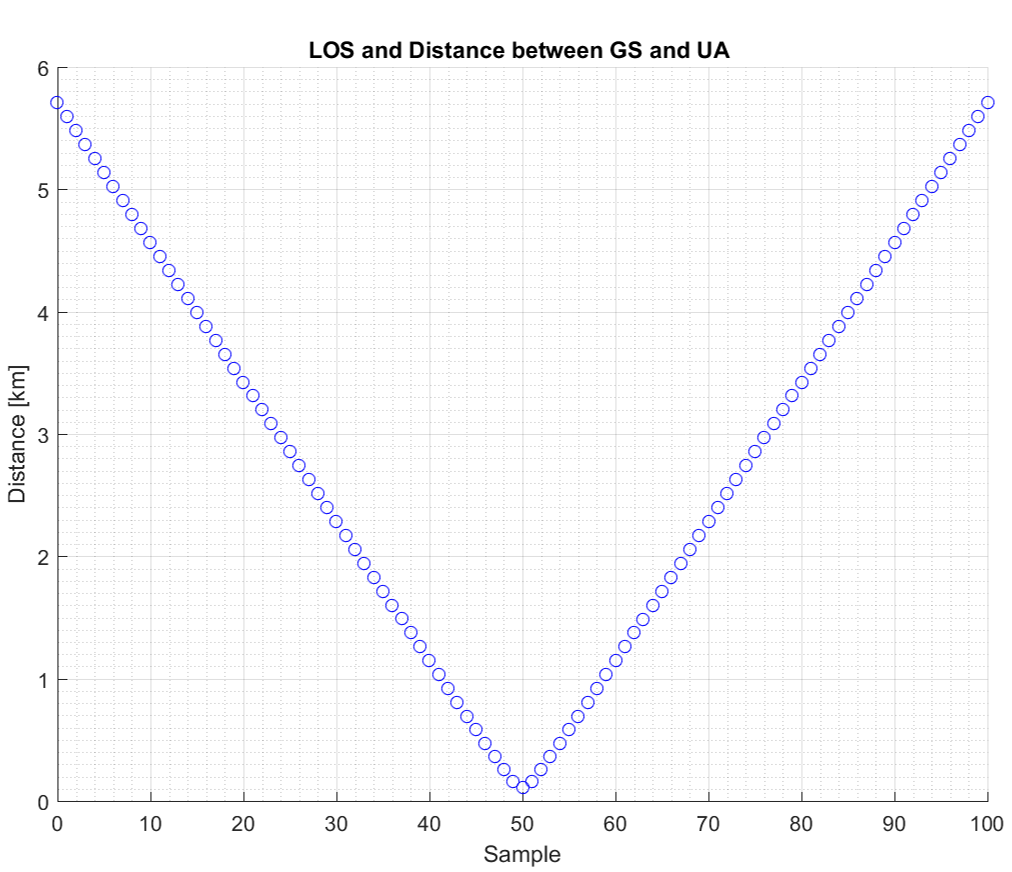
\includegraphics[scale=0.35]{figures/s3_los.png}}}
  \end{figure}

\end{frame}



\begin{frame}{Results}{Scenario 3 - Above the GS}

  \begin{block}{GS Tracking Angles}  
  
  \begin{figure}[H]
    \centerline{
    \subfigure[UAS Map]{
    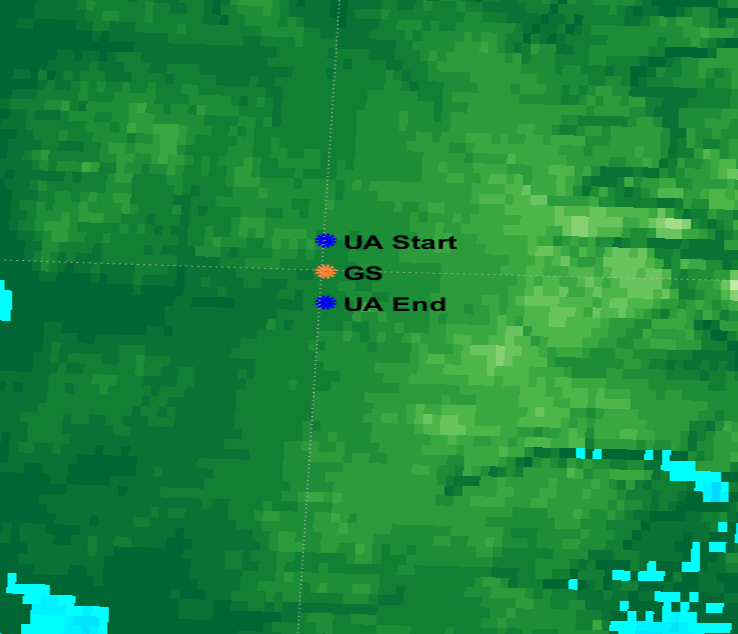
\includegraphics[scale=0.25]{figures/s3_zoom.png}}
    \hfill
    \subfigure[Azimuth and elevation angles of the antenna on the GS]{
    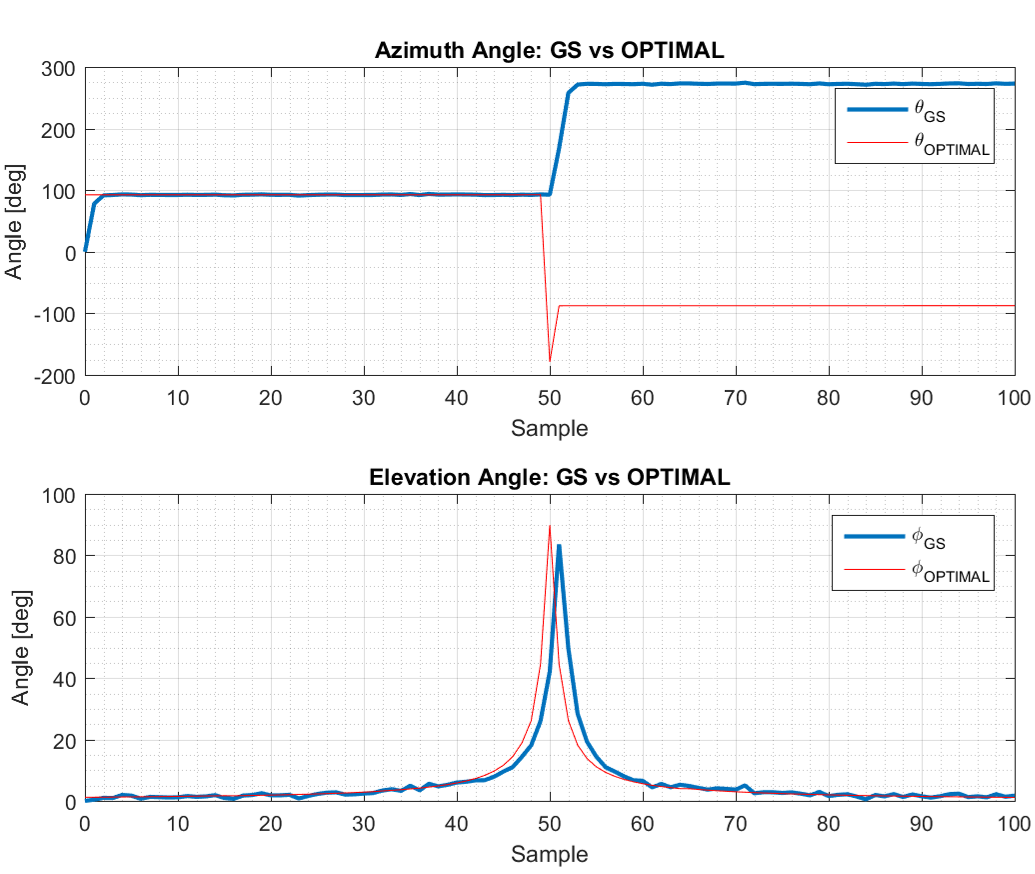
\includegraphics[scale=0.35]{figures/s3_gs.png}}}
  \end{figure}
  
  \end{block}

\end{frame}



\begin{frame}{Results}{Scenario 3 - Above the GS}

  \begin{block}{UA Tracking Angles}  
  
  \begin{figure}[H]
    \centerline{
    \subfigure[UAS Map]{
    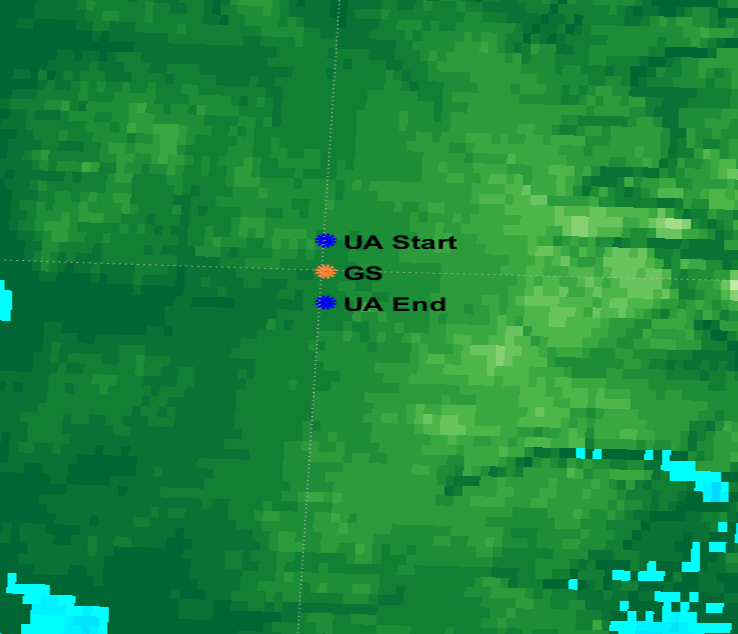
\includegraphics[scale=0.25]{figures/s3_zoom.png}}
    \hfill
    \subfigure[Azimuth and elevation angles of the antenna on the UA]{
    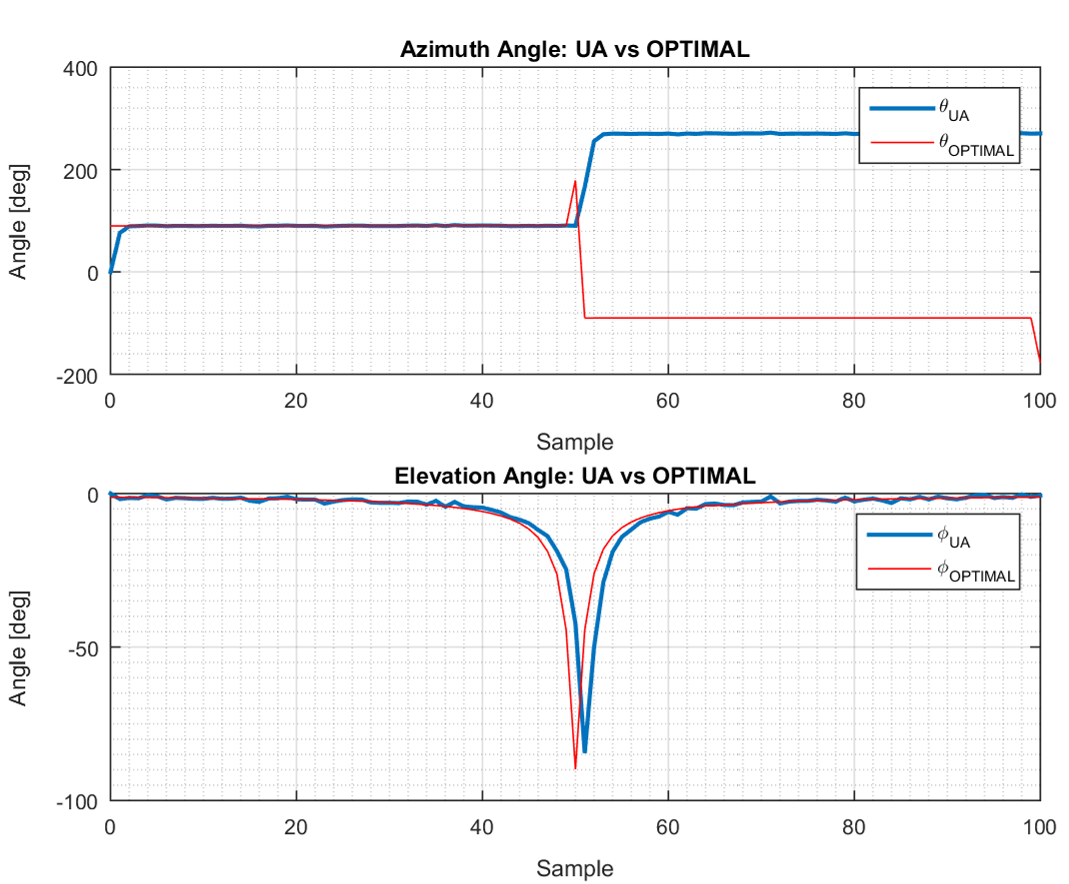
\includegraphics[scale=0.35]{figures/s3_ua.png}}}
  \end{figure}
  
  \end{block}

\end{frame}



\begin{frame}{Results}{Scenario 3 - Above the GS}

  \begin{block}{Signal Power}  
  
  \begin{figure}[H]
    \centerline{
    \subfigure[UAS Map]{
    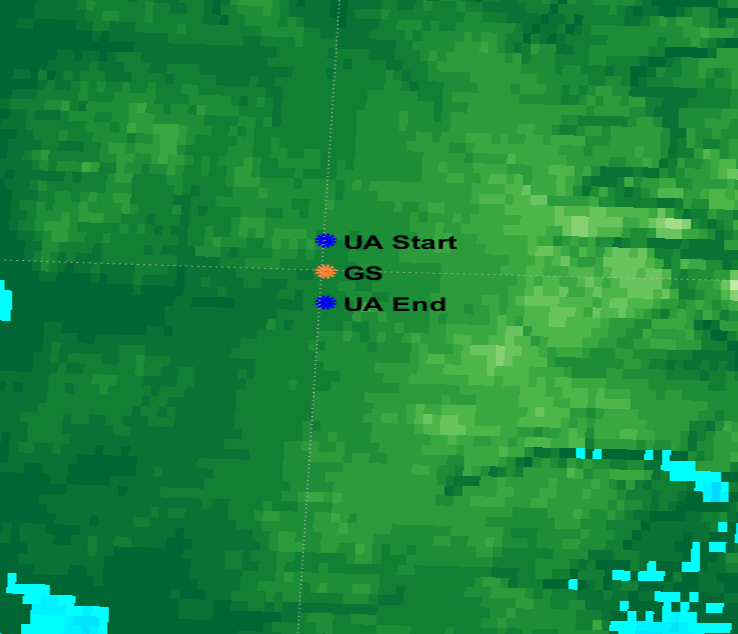
\includegraphics[scale=0.25]{figures/s3_zoom.png}}
    \hfill
    \subfigure[Power at the receiver]{
    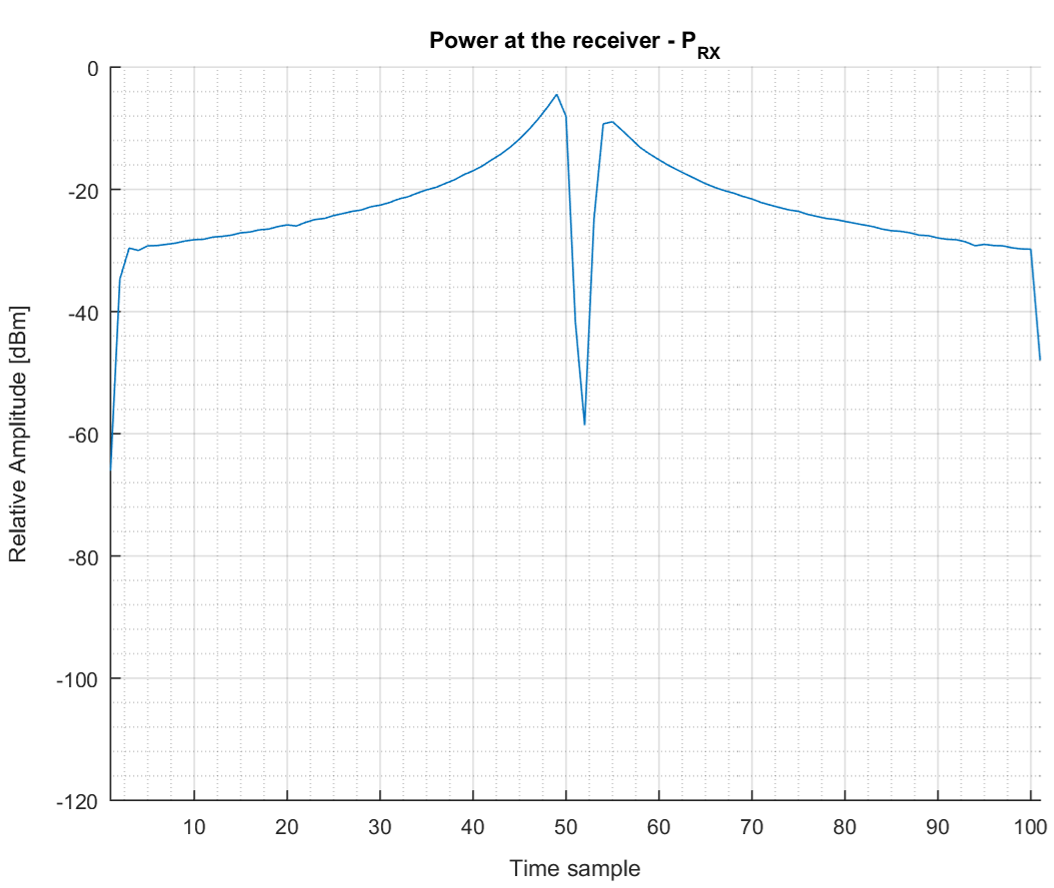
\includegraphics[scale=0.35]{figures/s3_power.png}}}
  \end{figure}
  
  \end{block}

\end{frame}

\subsection{Scenario 4}

\begin{frame}{Results}{Scenario 4 - Mountain}

  \begin{block}{Goal}
	Describing the movement of the antennas when the UA is flying behind a mountain.
  \end{block}

  \begin{figure}[H]
    \centerline{
    \subfigure[UAS Map]{
    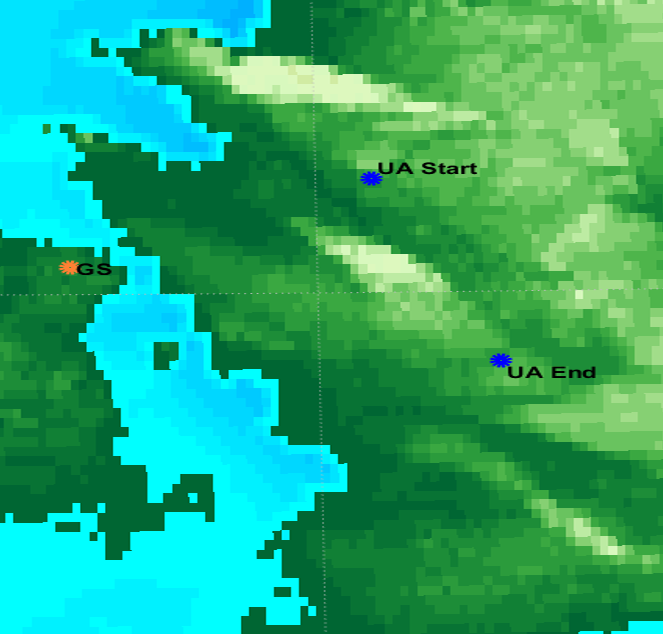
\includegraphics[scale=0.25]{figures/s4_zoom.png}}
    \hfill
    \subfigure[Distance between UA and GS]{
    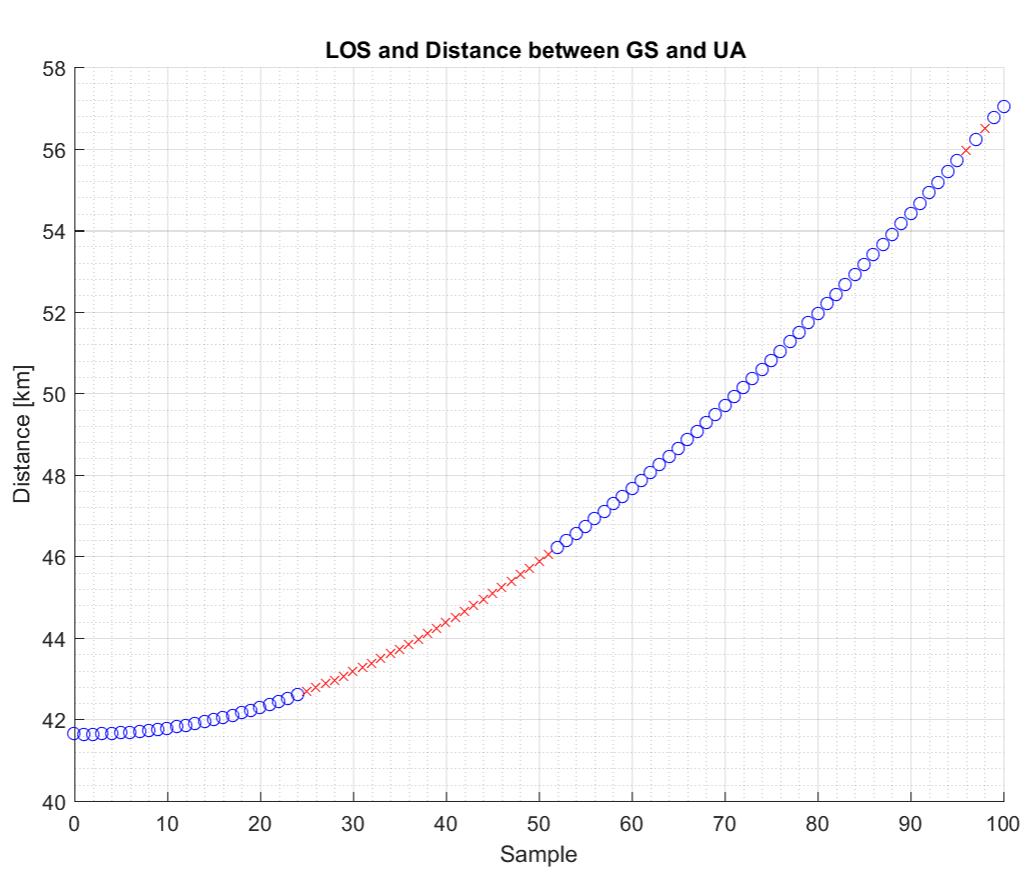
\includegraphics[scale=0.35]{figures/s4_los.png}}}
  \end{figure}

\end{frame}



\begin{frame}{Results}{Scenario 4 - Mountain}

  \begin{block}{GS Tracking Angles}  
  
  \begin{figure}[H]
    \centerline{
    \subfigure[UAS Map]{
    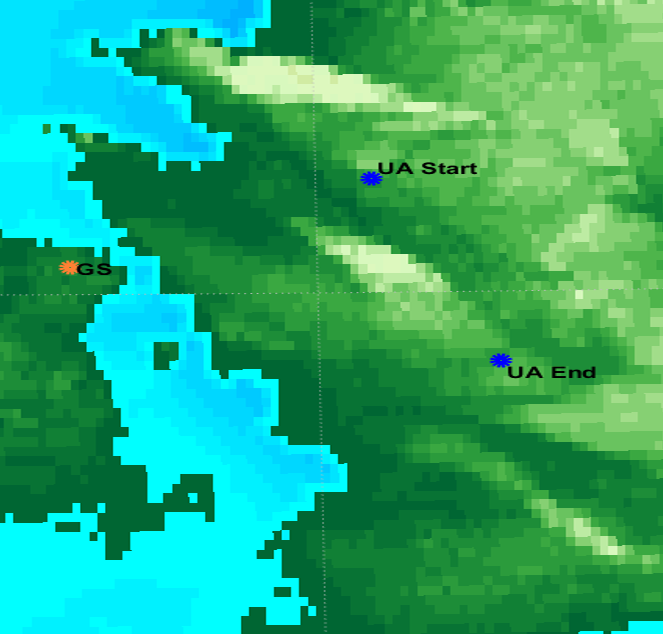
\includegraphics[scale=0.25]{figures/s4_zoom.png}}
    \hfill
    \subfigure[Azimuth and elevation angles of the antenna on the GS]{
    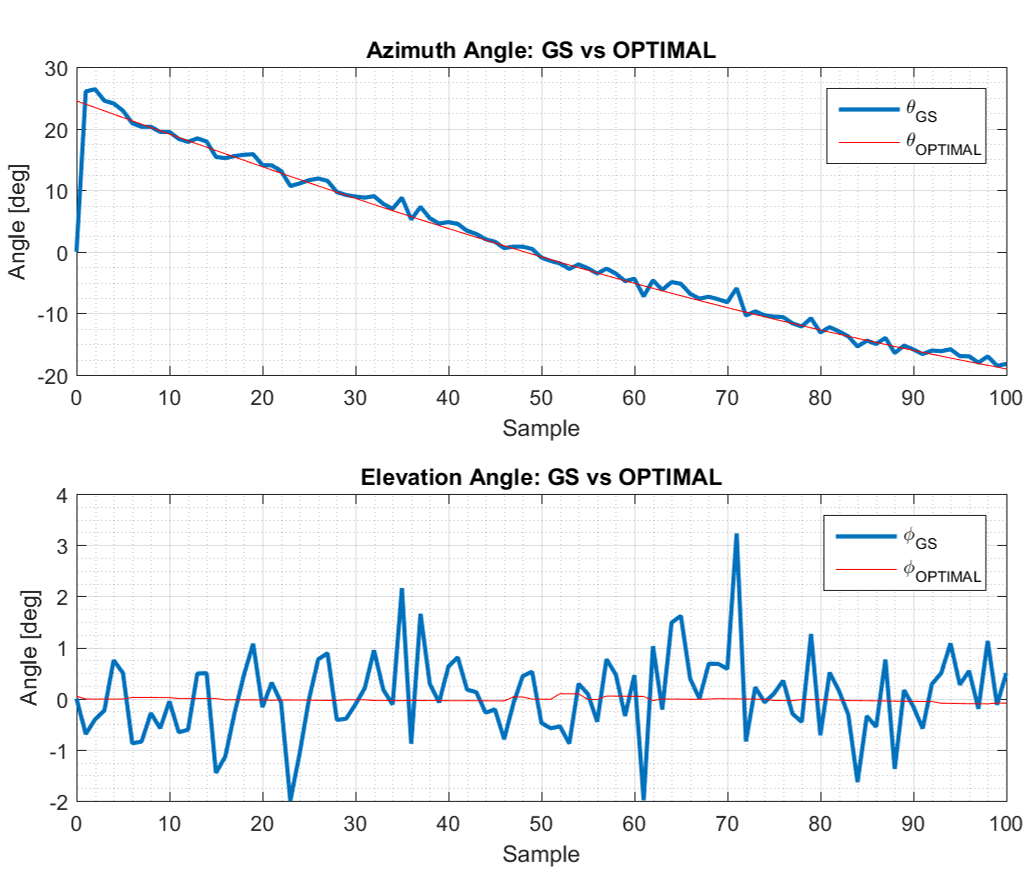
\includegraphics[scale=0.35]{figures/s4_gs.png}}}
  \end{figure}
  
  \end{block}

\end{frame}



\begin{frame}{Results}{Scenario 4 - Mountain}

  \begin{block}{UA Tracking Angles}  
  
  \begin{figure}[H]
    \centerline{
    \subfigure[UAS Map]{
    \includegraphics[scale=0.25]{figures/s4_zoom.png}}
    \hfill
    \subfigure[Azimuth and elevation angles of the antenna on the UA]{
    \includegraphics[scale=0.35]{figures/s4_ua.png}}}
  \end{figure}
  
  \end{block}

\end{frame}



\begin{frame}{Results}{Scenario 4 - Mountain}

  \begin{block}{Signal Power}  
  
  \begin{figure}[H]
    \centerline{
    \subfigure[UAS Map]{
    \includegraphics[scale=0.25]{figures/s4_zoom.png}}
    \hfill
    \subfigure[Power at the receiver]{
    \includegraphics[scale=0.35]{figures/s4_power.png}}}
  \end{figure}
  
  \end{block}

\end{frame}


\section{Conclusion}
\chapter{Conclusion}\label{ch:conclusion}
In case you have questions, comments, suggestions or have found a bug, please do not hesitate to contact me. You can find my contact details below.
  \begin{center}
    Jesper Kjær Nielsen\\
    \href{mailto: jkn@es.aau.dk}{jkn@es.aau.dk}\\
    \href{http://kom.aau.dk/~jkn}{http://kom.aau.dk/\textasciitilde jkn}\\
    Fredrik Bajers Vej 7\\
    9220 Aalborg Ø
  \end{center}



% list of the themes and options
% {\setbeamercolor{frametitle}{use=structure,fg=structure.fg,bg=white}
% \begin{frame}{User Interface}{Loading the Theme and Theme Options}
%   \begin{block}{The Color Theme}
%     You can load the color theme directly by\\
%     {\tt \textbackslash usecolortheme[<options>]\{AAUsidebar\}}\\
%     Currently, the only theme option is
%     \begin{itemize}
%       \item {\tt lightheaderbg}: use a light header background (currently, it is white). 
%     \end{itemize}
%     This option creates the light header used on this slide.
%   \end{block}
%   \pause
%   \begin{block}{The Color Element {\tt AAUsidebar}}
%     The color theme defines a new beamer color element named {\tt AAUsidebar} whose foreground and background colors are
%     \begin{itemize}
%       \item fg: {\usebeamercolor[fg]{AAUsidebar}light blue (\{RGB\}\{194,193,204\})}
%       \item bg: {\usebeamercolor[bg]{AAUsidebar}dark blue (\{RGB\}\{33,26,82\})}
%     \end{itemize}
%     You can use these colors in the standard beamer way by using the command
%     {\tt \textbackslash usebeamercolor[<fg or bg>]\{AAUsidebar\}}. See the beamer manual for instructions.
%   \end{block}
% \end{frame}
% }
%%%%%%%%%%%%%%%%

{\aauwavesbg
\begin{frame}[plain,noframenumbering]
  \finalpage{Thank you for flying with us!}
\end{frame}}
%%%%%%%%%%%%%%%%

\end{document}
